\documentclass[a4paper,11pt,oneside]{article}

\usepackage[utf8]{inputenc}
\usepackage[a4paper,top=3cm,bottom=3cm,left=3cm,right=3cm]{geometry}
\renewcommand{\familydefault}{\sfdefault}
\usepackage{helvet}
\usepackage[ruled,vlined]{algorithm2e}
\usepackage{amsmath}
\usepackage{float}
\usepackage{tikz}
\usepackage{amsthm}
\usepackage{csquotes}
\usepackage{tabularx}
\usepackage[T1]{fontenc}
\usepackage{array}
\usepackage[english]{babel}     %% typographie française
\usepackage[backend=bibtex,style=numeric,language=english]{biblatex}
\usepackage{parskip}		%% blank lines between paragraphs, no indent
\usepackage[margin=1cm]{caption}%% give long captions a margin
\usepackage{subcaption}
\usepackage{booktabs}           %% typesetting nice tables
\usepackage{graphicx}	%% include graphics, preferrably pdf
\usepackage{hyperref}	%% many PDF options can be set here
\pdfadjustspacing=1		%% force LaTeX-like character spacing

\newcommand{\minus}{\scalebox{0.9}[1.0]{$-$}} %% my custom minus sign

\newenvironment{conditions}
  {\par\vspace{\abovedisplayskip}\noindent\begin{tabular}{>{$}l<{$} @{${}={}$} l}}
  {\end{tabular}\par\vspace{\belowdisplayskip}}

\newcommand{\myname}{Otmane Sabir}
\newcommand{\mytitle}{Accelerated Ray Tracing of Constructive Solid Geometry}
\newcommand{\mysupervisor}{Prof. Dr. Sergey Kosov}

\hypersetup{
  pdfauthor = {\myname},
  pdftitle = {\mytitle},
  pdfkeywords = {},
  colorlinks = {true},
  linkcolor = {blue},
  citecolor = {blue}	
}

\addbibresource{references.bib}

\begin{document}
\pagenumbering{roman}

\thispagestyle{empty}

\begin{flushright}
	
\includegraphics[scale=0.8]{bsc-logo}
\end{flushright}
\vspace*{40mm}
\begin{center}
	\huge
	\textbf{\mytitle}
\end{center}
\vspace*{4mm}
\begin{center}
	\Large by
\end{center}
\vspace*{4mm}
\begin{center}
	\LARGE
	\textbf{\myname}
\end{center}
\vspace*{20mm}
\begin{center}
	\Large
	Bachelor Thesis in Computer Science
\end{center}
\vfill
\begin{flushleft}
	\large
	Submission: \today \hfill Supervisor: \mysupervisor \\
	\rule{\textwidth}{1pt}
\end{flushleft}
\begin{center}
	Jacobs University Bremen $|$ Department of Computer Science and Electrical Engineering
\end{center}

\newpage
\thispagestyle{empty}

\subsection*{English: Declaration of Authorship}
 
I hereby declare that the thesis submitted was created and written
solely by myself without any external support. Any sources, direct
or indirect, are marked as such. I am aware of the fact that the
contents of the thesis in digital form may be revised with regard to
usage of unauthorized aid as well as whether the whole or parts of
it may be identified as plagiarism. I do agree my work to be entered
into a database for it to be compared with existing sources, where
it will remain in order to enable further comparisons with future
theses. This does not grant any rights of reproduction and usage,
however.

This document was neither presented to any other examination board
nor has it been published.

\subsection*{German: Erklärung der Autorenschaft (Urheberschaft)}
 
Ich erkläre hiermit, dass die vorliegende Arbeit ohne fremde Hilfe
ausschließlich von mir erstellt und geschrieben worden ist. Jedwede
verwendeten Quellen, direkter oder indirekter Art, sind als solche
kenntlich gemacht worden. Mir ist die Tatsache bewusst, dass der
Inhalt der Thesis in digitaler Form geprüft werden kann im Hinblick
darauf, ob es sich ganz oder in Teilen um ein Plagiat handelt. Ich
bin damit einverstanden, dass meine Arbeit in einer Datenbank
eingegeben werden kann, um mit bereits bestehenden Quellen
verglichen zu werden und dort auch verbleibt, um mit zukünftigen
Arbeiten verglichen werden zu können. Dies berechtigt jedoch nicht
zur Verwendung oder Vervielfältigung.

Diese Arbeit wurde noch keiner anderen Prüfungsbehörde vorgelegt
noch wurde sie bisher veröffentlicht.

\vspace{20mm}

Date, Signature

\newpage

\section*{Acknowledgements}

The journey towards this thesis has been circuitous. Its completion is thanks to the special people who challenged, supported, directed, and drove me along the way.

I am tremendously fortunate for my supervisor, Professor Dr. Sergey Kosov, whose expertise was invaluable in the progress of this research. Your theoretical and practical experience remains a central part in understanding the research, architecting the implementation, and analyzing the results.  Your stellar feedback pushed me to sharpen my thinking and opened up different perspectives concerning several matters. I am grateful for the inspiration you have been able to instill in all steps of this study.

Additionally, I am deeply indebted to my parents, my sister, and grandmother for their wise guidance, thoughtful words, and tender care. You are always there for me. Finally, I could not have completed this dissertation without the support of my friends who continuously taught me how to embrace change and strive for the best.  

\newpage

\section*{Abstract}
  
% TODO: add this reference
% http://www.cs.unc.edu/~fuchs/publications/VisSurfaceGeneration80.pdf
   
  
(target size: 15-20 lines)

\newpage
\tableofcontents

\clearpage
\pagenumbering{arabic}

\section{Introduction}
  
Constructive Solid Geometry (CSG) is a method used in computer graphics, computer-aided design, generic modeling languages, and numerous other applications to construct complex geometries from simple primitives or polyhedral solids through the use of boolean operators, namely union ($\cup$),  intersection ($\cap$), and difference ($\minus$). Figure \ref{sec1:set-operations-examples} respectively shows union, intersection, and difference operations. The approach grows especially appealing when implemented in a ray tracing system as the core intricacy renders performing arithmetic logic on a pair of uni-dimensional rays. Nonetheless, most current ray tracing systems generally suffer from the detriment of the expensive object space intersection computation, and the generic CSG algorithms suffer immensely from their computational complexity, making it very difficult to integrate into operating rendering engines. Therefore, this research concentrates on constructive solid geometry and possible means of acceleration.
  
\begin{figure}[ht]
	\centering
	\begin{subfigure}[b]{0.3\textwidth}
		\centering
		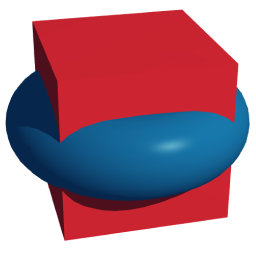
\includegraphics[width=\textwidth]{section1/union.png}
		\caption{Union.}
		\label{sec1:union}
	\end{subfigure}
	\hfill
	\begin{subfigure}[b]{0.3\textwidth}
		\centering
		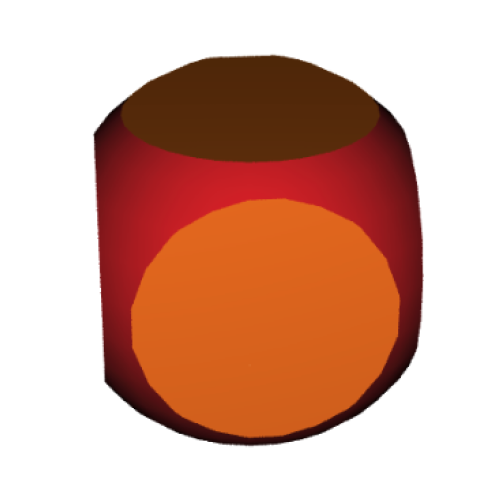
\includegraphics[width=\textwidth]{section1/intersection.png}
		\caption{Intersection.}
		\label{sec1:intersection}
	\end{subfigure}
	\hfill
	\begin{subfigure}[b]{0.3\textwidth}
		\centering
		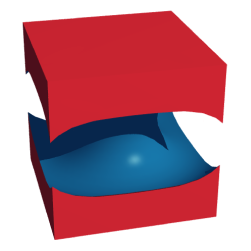
\includegraphics[width=\textwidth]{section1/difference.png}
		\caption{Difference.}
		\label{sec1:difference}
	\end{subfigure}
	\hfill
	\caption{Examples of set operations on a mesh torus and box.}
	\label{sec1:set-operations-examples}
\end{figure}

  
\subsection{Rendering Algorithms}
  
Rendering digital photorealistic or non-photorealistic images has been a topic of study since the late 1960s \cite{INITIAL_RENDERING}. Since then, various algorithms came forth that allow achieving different results depending on the required conditions. Inherently all these algorithms strive to solve the same underlying problem by trading-off different aspects, namely speed and realism. This problem is known as the hidden surface problem \cite{hidden-surface-problem}. The hidden surface problem is determining the visible objects in space from a certain point of view. There are two general methods, object-space methods, which try to start from the object space and project the geometries onto the 2D raster, or the image-space ones, which perform the opposite by tracing a ray through each pixel and attempting to locate the closest intersection of that ray with the geometries in the scene. The two methods then give birth to the pair of most famous and widely adopted rendering algorithms: rasterization and ray tracing.
  
\subsubsection{Rasterization}
    
Rasterization has very quickly become the predominant approach for interactive applications because of its initially low computational requirements, its massive adoption in most hardware solutions, and later by the ever-increasing performance of dedicated graphics hardware. The use of local, per-triangle computation makes it well suited for a feed-forward pipeline. However, the rasterization algorithm has many trade-offs. To name a few: handling of global effects such as reflections and realistic shading, and limitations to scenes with meshed geometries \cite{rasterization_scratch_pixel}. 
    
\subsubsection{Ray Tracing}
     
Ray tracing simulates the photographic process in reverse. For each pixel on the screen, we shoot a ray and identify objects that intersect the ray. A ray-tracing algorithm makes use of four essential components: the camera, the geometry, the light sources, and the shaders. These components can have different varieties, to state a few, orthographic and perspective cameras, unidirectional and area light sources, and Phong and chrome shaders. Hence, it allows achieving several outcomes depending on the necessities. The main downside has been computational time and the constraints of using such an algorithm in interactive applications. However, ray tracing parallelizes efficiently and trivially. Thus it takes advantage of the continuously rising computational power of the hardware. Many applications have successfully produced real-time ray tracing algorithms and allow for highly photorealistic results in interactive applications \cite{RT_RT1, RT_RT2}.
    
  
\subsection{Geometric Representations}
\label{sec:geometric_represections}

When it comes to computer graphics, we can find numerous types of geometry descriptions \cite{SOLIDREP_5, SOLIDREP_1, SOLIDREP_2, SOLIDREP_3, COMPUTING_SURVEYS,SOLIDREP_4}. Many solutions exist that enable the simple conversion between these geometric formats \cite{steuer_2012}. However, there are predominantly two different representations in most geometric modeling systems \cite{COMPUTING_SURVEYS}: boundary representations - commonly known as B-Rep or BREP - and constructive solid geometry - CSG. Each one of these representations brings forward different advantages, disadvantages, and limitations.
    
\subsubsection{Boundary Representation}
    
Boundary representations are indirect definitions of solids in space using their boundary or limit. This representation is usually a hierarchical composition of different dimensionally complex parts. On the very top, we have definitions of two-dimensional faces, which build on uni-dimensional edges that are subsequently built on dimensionless vertices (Figure \ref{fig2:brep_3d_rect}). A BREP with non-curvilinear edges and planar faces is called a polygon mesh. A triangle is the simplest polygon and has the excellent property of always being co-planar. Additionally, polygons of any complexity are representable by a set of triangles. These qualities make triangular meshes a fundamental component in BREPs. The representations built on triangles are also highly optimized for fast operations. Therefore, we will mainly deal with triangular meshes in OpenRT, though it does offer descriptions for tetragon (quadrilateral) meshes.
    
    
\begin{figure}[ht]
	\begin{center}
		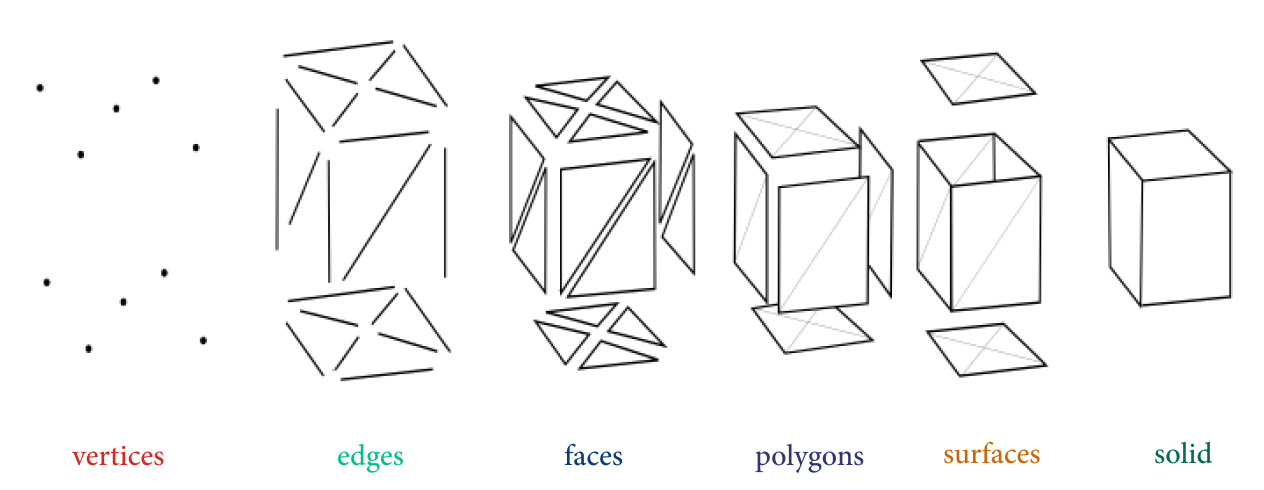
\includegraphics[width=.8\textwidth]{section1/brep-overview.png}
	\end{center}
	\caption{Sample BREP of a 3D hyper-rectangle \cite{wikipedia_2021_mesh_rep}}
	\label{fig2:brep_3d_rect}
\end{figure}
    
\subsubsection{Constructive Solid Geometry}

Constructive solid geometry takes basis on the fundamental premise that any complex physical object is obtainable from a set of primitive geometries and the base boolean operations. CSG is radically different from BREPs as it does not collect any topological information but instead evaluates the geometries as needed by the case scenario. In other words, there is no explicit description of the boundary of the solid. Contrary to BREPs,  CSG representations are quickly modified and manipulated since incremental changes do not trigger re-computation and evaluation of the boundary of a geometry. Therefore, no topological changes occur when adjusting the geometries. The latter makes it an attractive solution as it provides a high-level specification of the objects in space and permits significantly more straightforward modification and manipulation. In the general constructive solid geometry description, the solids are put in a binary tree, referred to as the CSG tree (Figure \ref{sec3.1:sample-csg-tree}). The root node is the complete composite geometry. The leaf nodes depict the base geometries (cubes, spheres, cylinders, tori, cones, and polygon meshes\footnote{Polygon meshes are usually not considered in CSG algorithms; however, the implementation discussed here allows such flexibility.}) used in the composition. Every node in the tree, besides the leaf nodes, expresses another complete solid and contains information of the set operation of that node.
    
In the OpenRT library implementation, we follow a different approach to allow the use of BREPs as leaf nodes. This gives the flexibility of creating more complex geometries and allowing for nesting of combinatorial geometries inside each other. In a naive implementation, this operation can be costly; however, by using certain spatial indexing structures, each node can be represented as a binary space partitioning tree.
  
\begin{figure}[ht]
	\begin{center}
		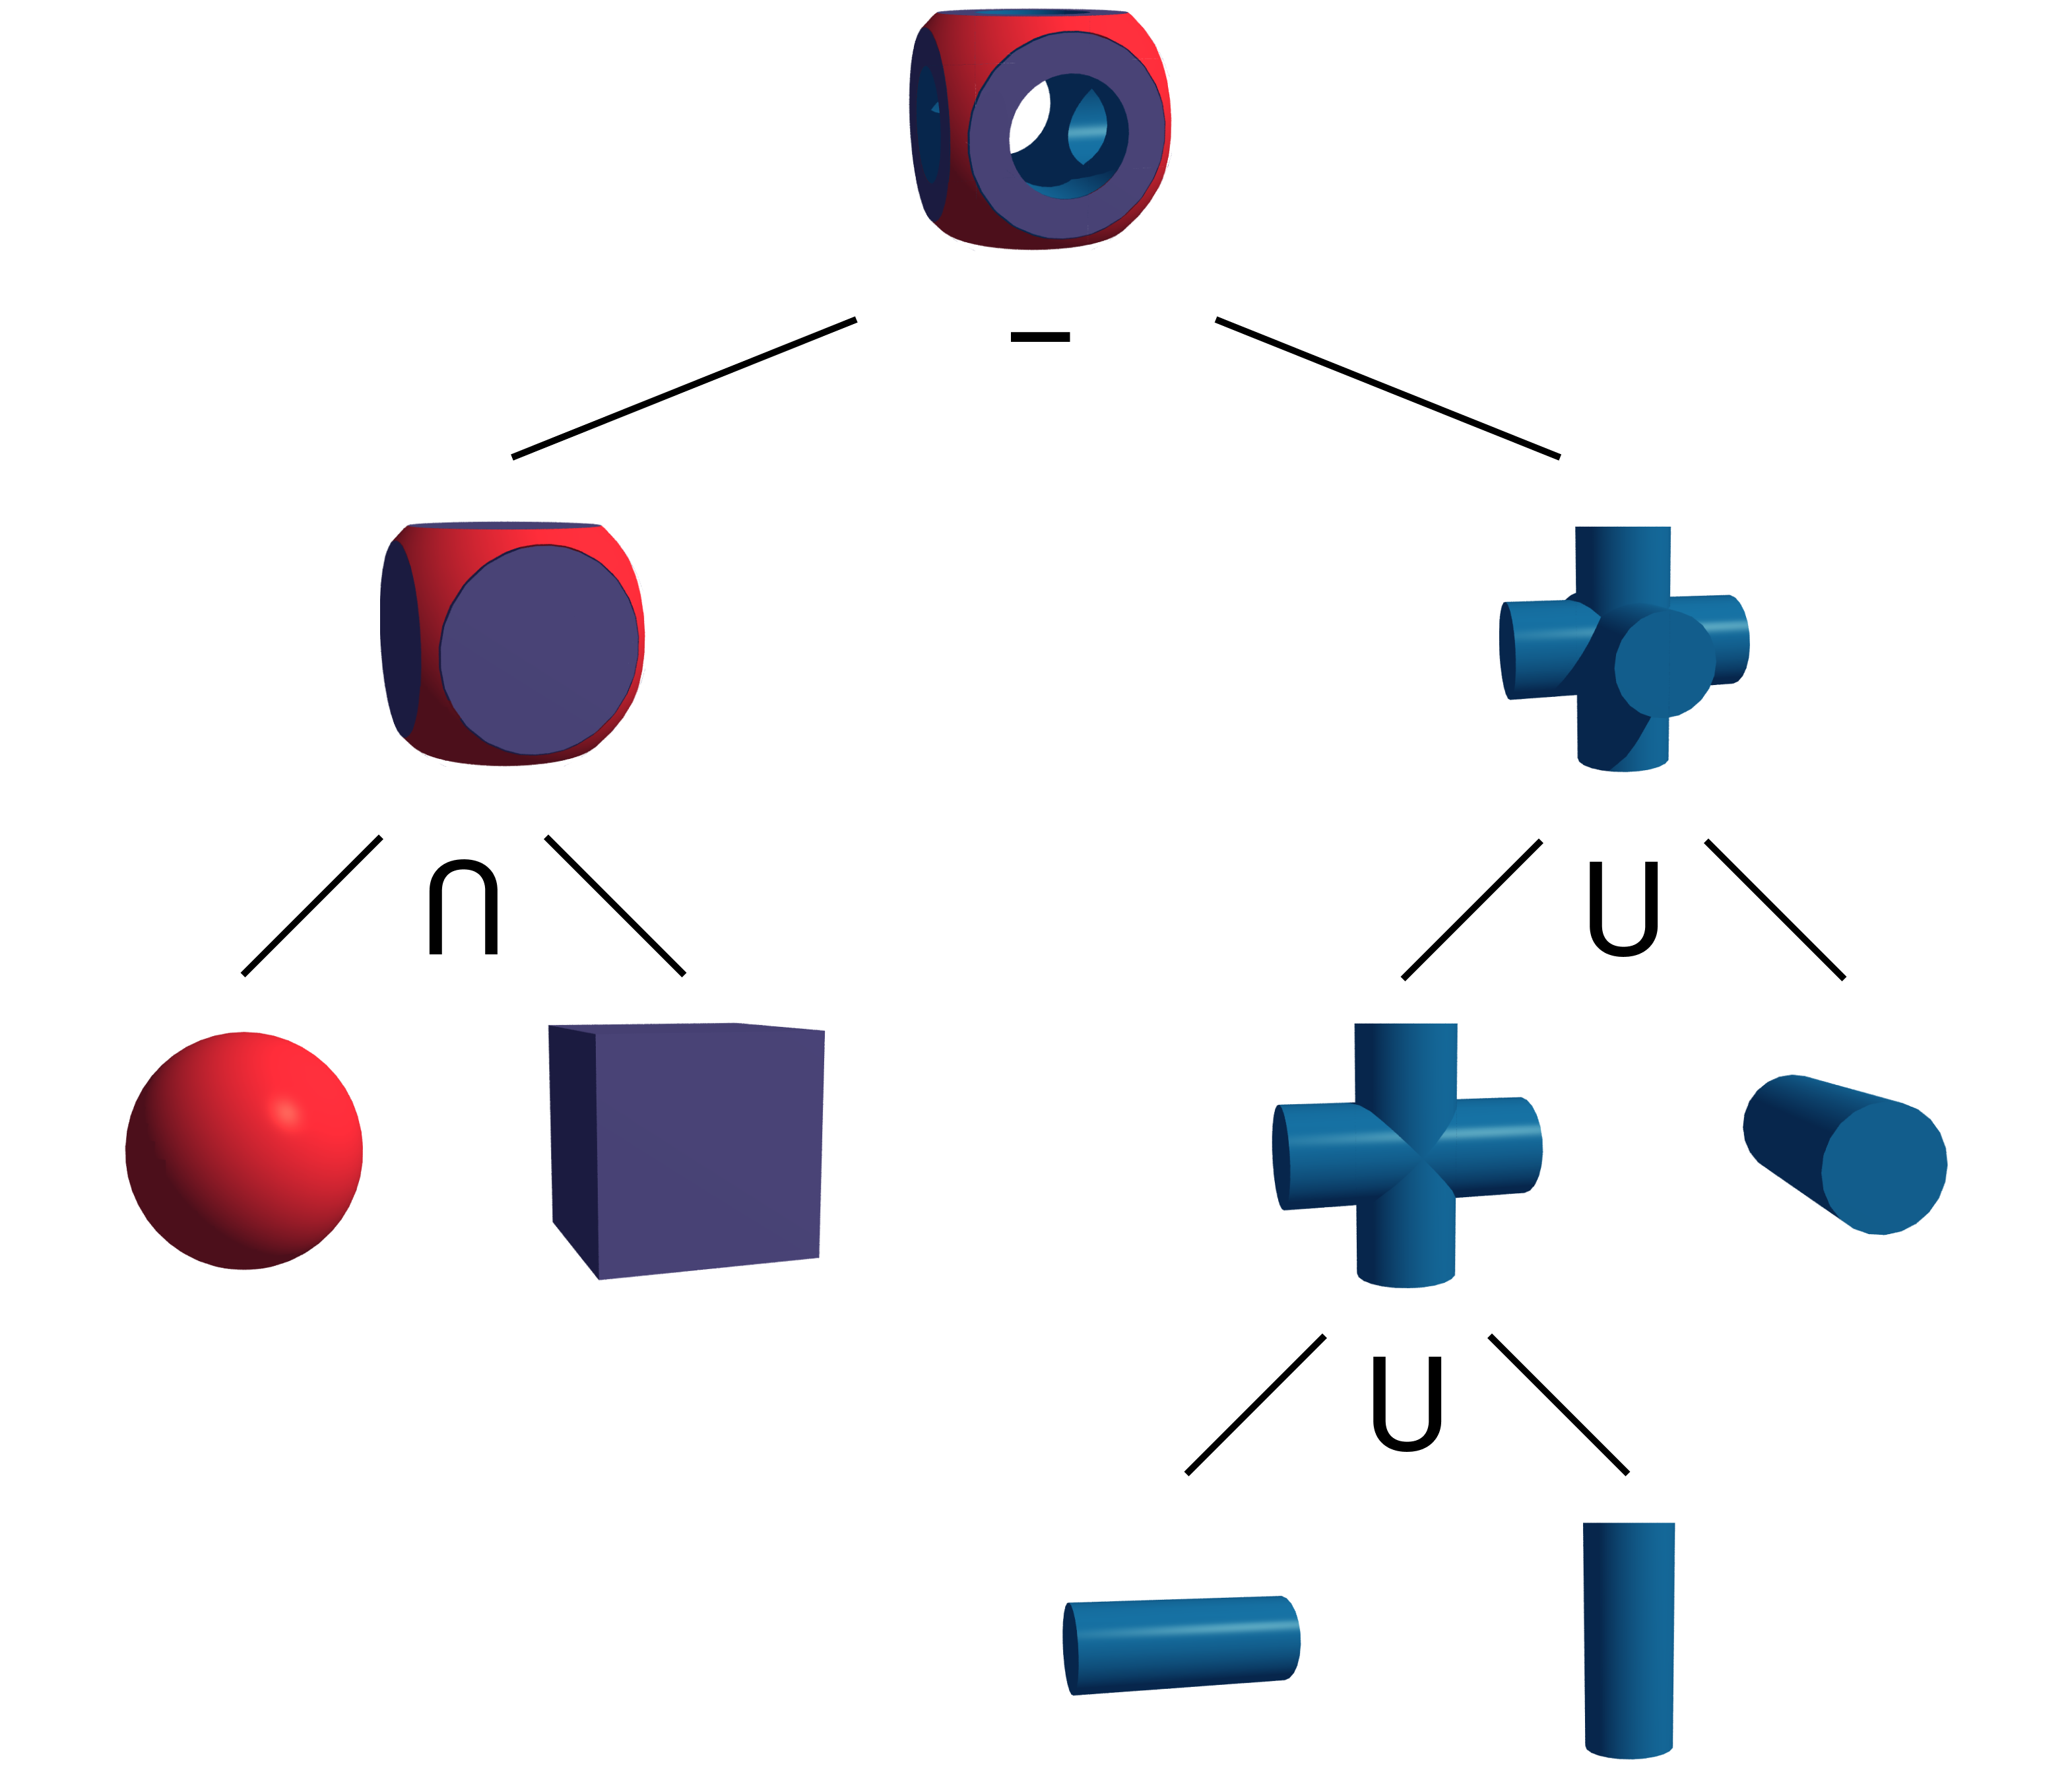
\includegraphics[width=0.7\textwidth]{section1/sample-csg-tree.png}
	\end{center}
	\caption{Sample representation of a CSG tree.}
	\label{sec3.1:sample-csg-tree}
\end{figure}
  
\subsection{Overview}
  
We present this CSG implementation in six sections. 1. Introduction;  2. Related Works; 3. Constructive Solid Geometry; 4. Optimization; 5. Evaluation of the results; 6. Extensions \& Conclusions.

The first section was the previous introduction laying a foundation to a few topics we will be addressing. 
  
The second section presents works already done, the limitations of the proposed implementations, and solutions to problems related to CSG.
  
Section 3 defines the algorithm that performs the logic in the ray-tracing framework. We first introduce the ideas behind ray intersection. We then lay a mathematical foundation to boolean algebra and membership classification. Additionally, we dive into the detail of ray classification for constructively generated geometries. 
  
Section 4 discusses efficiency and optimization. The visible surface problem in ray tracing requires a lot of CPU time, and without any optimization, the CSG algorithm significantly increases the payload. Therefore, improvement is much needed to make this method usable and suitable for real-life applications. The speed is a function of the screen resolution and the geometry complexity (the number primitives (e.g., triangles) in the solid, and the number of nested geometries).
  
Section 5 describes the different implementations of the CSG algorithm with the various optimization techniques. The first is the naive implementation which we refer to as $NaiCSG$. The second is a variant that uses a binary space partitioning tree to solve the visible surface problem but still naively finds intersections inside the combinatorial geometry, which we will refer to as $BinCSG$. Lastly, we'll introduce our optimized algorithm which uses a binary space partition tree on the outside (solving the visible surface problem) and also inside each composite geometry to direct the rays towards the correct geometries, which we will refer to as $OptimCSG$. We conduct three types of tests. The primary one is a function of time and complexity of the geometry, as we monitor the rendering time following gradual increases in the detail level of two sphere meshes. The second computes the time taken to render a scene after covering different amounts of the view port. Third we also conduct a test to check the number of ray tests conducted per pixel. The final test computes the time variations after increasing the number of nested geometries present in the composite solid while crucially maintaining a consistent view port fill rate.
  
  
\section{Related Work}
  
I discuss below the techniques most related to ours. However, there is a tremendous body of work in this area and I cannot possibly provide an absolute overview. The goal is instead to outline similarities and differences with some of the widely adopted approaches for CSG modeling.

Constructive solid geometry has been a subject of study since the late 1970s. It was initially introduced in \cite{GEOMETRIC_MODELING_1977} as a digital solution to help in the design and production activities in the discrete goods industry, this marked the basis for formalizing the method.
  
A rigorous mathematical foundation of constructive solid geometry was later laid out in \cite{Requicha1978MathematicalFO}. The membership classification function, a generalization of the ray clipping method, is also thoroughly discussed and various formal properties are introduced.
  
A few years later it was revisited in \cite{ROTH1982109} where \citeauthor{ROTH1982109} et al. (\citeyear{ROTH1982109}) introduced ray casting as a basis for CAD solid modeling systems. Challenges of adequacy and efficiency of ray casting are addressed, and fast picture methods for interactive modeling are introduced to meet the challenges.
  
The focus then turned towards different optimizations of CSG algorithms in the setting of ray tracing. A simplistic single hit intersection algorithm is introduced in \cite{kensler_ray_2006}. This suggested mechanism reduces memory load and the number of computations performed for ray classification. Though limitations have to be respected since sub-objects must closed, non-self-intersecting, and have consistently oriented normals. However, this was later proven to be a solution that does not gracefully handle edge cases especially for the difference and intersection operations \cite{csg-xrt-renderer}.
  
A "slicing" approach is also proposed in \cite{lefebvre:hal-00926861}. Similar to our proposed solution combinations of meshes and analytical primitives through CSG operations are permissible. Nevertheless, this approach requires one boolean per primitive and a complete evaluation of the CSG expression in each step; therefore, making it simple but limited, and much better approaches are imaginable.

Bound definitions are also a popular way of significantly reducing the time required by CSG algorithms. If the ray and the geometric entities are bound, we first perform a test to see if the ray and the bounding volume around a geometric entity overlap. Only when the boxes overlap does one continue to test whether the ray and the entity do so as well. A submitted S-bounds algorithm is brought forth in \cite{sbounds_csg} as a means of acceleration in solid modeling and CSG.
  
Techniques that optimize various CSG rendering algorithms, namely the Goldfeather and the layered Goldfeather algorithm, and the Sequenced-Convex- Subtraction (SCS) algorithm are advanced in \cite{hardware_accelerated_image_based_csg.}. Although the work represents a significant improvement towards real-time image-based CSG rendering for complex models,  the main focus is on hardware acceleration.
  

\section{Constructive Solid Geometry}
    
\subsection{Ray Intersection}
\label{section:ray-intersection}

Ray intersection is the essence of all ray tracing systems. We supply the system a ray as input and obtain knowledge on how the ray intersects solids in the scene as an output. In ray tracing engines, one only necessitates computing the nearest intersection to assess the given scene. However, when evaluating CSG models, we require all of the intersections with a geometry to arrange the ray intersections. With knowledge of all the information in the scene - essentially the camera model and the solids - an evaluation of these intersections are executed with each returning the latter information:

\begin{conditions}
	\vec{o}     & the origin of the ray (e.g., camera model origin). \\
	\vec{d}     & the direction of the ray (e.g., direction from camera origin to pixel in raster). \\
	t     &  the distance to either the closest or furthest intersection. \\
	prim    &  a pointer holding surface information of the intersected primitive. 
\end{conditions}

We can distinguish two types of ray intersections \cite{rasterization_scratch_pixel}. Firstly, ray-primitive intersection tests on convex primitives such as blocks, cylinders, cones, and spheres. Because the primitives are analytically defined, the solution is solving the analytic intersection equation. Consequently, this means that the intersection solution is primitive-specific. Many resources providing the analytical solutions are available \cite{ray_primitive_intersections}.
Second, we encounter the more generic solid-ray intersection. As we have previously defined in the introduction, a solid is often a boundary representation composed of several triangles. Hence, the main intricacy in ray-solid intersection renders iterating over all primitives and reducing the problem to $n$ ray-primitive intersection tests with $n$ being the number of primitives (e.g., triangles) in the solid.
We can consider the ray-solid intersection as a more general form of ray-primitive intersection since a primitive is always representable as a solid bearing a single surface. The interesting consequence of such an abstraction is that if we test a ray in the scene, the computation for determining ray intersection can be generalized to:

\begin{algorithm}[H]
	\SetAlgoLined
	\KwResult{$arr$ array of intersections}
	$i$ = 0\;
	\For{every primitive in the solid}{	
		solve the ray-primitive equations\;
		\uIf{intersection exists}{
			$arr[i]$ = current intersection\;
			$i$ = $i + 1$\;
		}
	}
	\caption{Ray-solid intersection checks.}
\end{algorithm}

The ray-solid intersection test has four possible outcomes:
\begin{enumerate}
	\item The ray misses the solid (Figure \ref{sec3.1:miss-intersection}).
	\item The ray is tangent to the solid (Figure \ref{sec3.1:tangent-intersection}).
	\item The ray enters and exists the solid (Figure \ref{sec3.1:complete-intersection}).
	\item The ray is inside/on the face of a solid and has one intersection. (Figure \ref{sec3.1:inside-intersection})
\end{enumerate}


\begin{figure}[ht]
	\centering
	\begin{subfigure}[b]{0.4\textwidth}
		\centering
		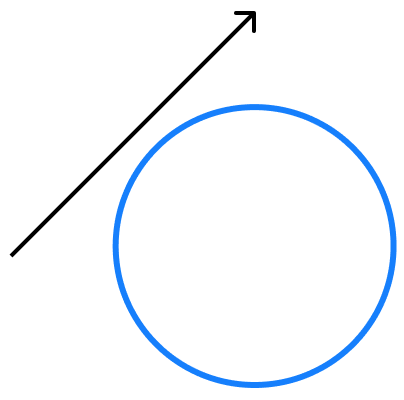
\includegraphics[width=\linewidth]{section3/3.1/intersection-miss.png}
		\caption{Miss intersection.}
		\label{sec3.1:miss-intersection}
	\end{subfigure}
	\hfill
	\begin{subfigure}[b]{0.4\textwidth}
		\centering
		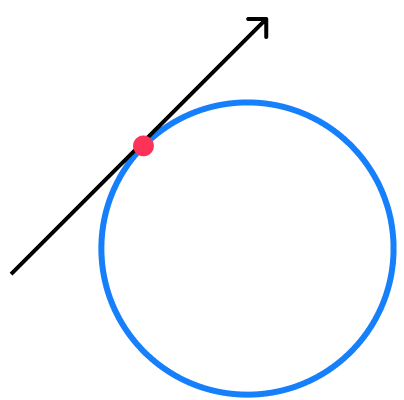
\includegraphics[width=\linewidth]{section3/3.1/intersection-tangent.png}
		\caption{Tangent intersection.}
		\label{sec3.1:tangent-intersection}
	\end{subfigure}
	\medskip
	\begin{subfigure}[b]{0.4\textwidth}
		\centering
		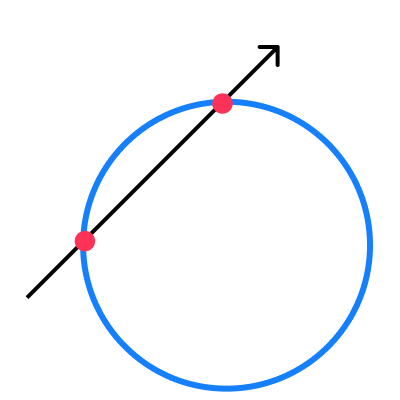
\includegraphics[width=\linewidth]{section3/3.1/intersection-in-out.png}
		\caption{Complete intersection.}
		\label{sec3.1:complete-intersection}
	\end{subfigure}
	\hfill
	\begin{subfigure}[b]{0.4\textwidth}
		\centering
		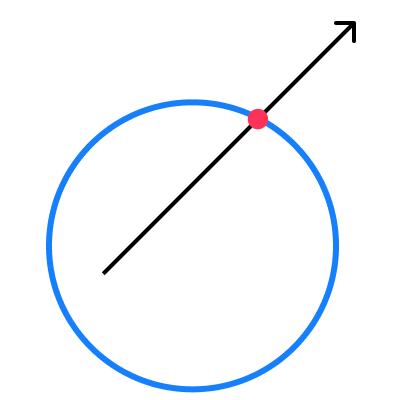
\includegraphics[width=\linewidth]{section3/3.1/intersection-out.png}
		\caption{Inside intersection.}
		\label{sec3.1:inside-intersection}
	\end{subfigure}
	\caption{Different ray intersection cases on a disk.}
	\label{sec3.1:intersection-cases}
\end{figure}


The first case is self-evident. In case 3, we compute both the entering and exiting points normally. The second and fourth case are more intricate to determine as we need to understand whether the intersection is inside or outside of the solid. We can find that by checking the orientation of the surface normal, $\vec{N}$, at the intersected point. If $\vec{N}\cdot\vec{d} < 0$, then the intersection point is outside. Otherwise, it is inside of the solid.

\subsection{Mathematical Formulations}
  
Constructive solid geometry is largely grounded in modern Euclidean geometry and the general topology of subsets of three-dimensional Euclidean space $E^3$ \cite{Requicha1978MathematicalFO}. As one cannot design a reliable geometric algorithm in the absence of a clear mathematical statement of the problem to be solved, I will be treating a few mathematical formulations. Topology and set theory have been intensively discussed previously in \cite{Requicha1978MathematicalFO}, \cite{tilove1977a},\cite{lachlan_srebrny_zarach_1977}, and many other resources. Hence, I will be mainly focusing on definitions and properties that interest us. Formal proofs of the introduced properties are also available in the before-mentioned resources.
  
\subsubsection{Set Algebra}
  
\theoremstyle{definition}
\newtheorem{definition}{Definition}[section]
  
\theoremstyle{property}
\newtheorem{property}{Property}[section]
    
\theoremstyle{remark}
\newtheorem*{remark}{Remark}
      
\begin{definition}[Set Operations]
	Assume that $X$ and $Y$ are subsets of a universe $W$. We can use the following standard notations:
			      
	\begin{equation} \label{eq:union}
		X \cup Y
	\end{equation}
	\begin{equation} \label{eq:intersection}
		X \cap Y
	\end{equation}
	\begin{equation} \label{eq:difference}
		X \minus Y
	\end{equation}
			        
	Where \eqref{eq:union}, \eqref{eq:intersection}, and \eqref{eq:difference} respectively denote the union, intersection, and difference of the subsets $X$ and $Y$.	        
\end{definition}

\begin{property}
	\label{prop:3.1}
	Union and intersection operations are commutative. \cite{mansfield_1987}
	\begin{equation*}
		X \cup Y = Y \cup X
	\end{equation*}
	\begin{equation*}
		X \cap Y = Y \cap X
	\end{equation*}
\end{property}
        
\begin{property}
	\label{prop:3.2}
	Union and intersection operations are distributive over themselves and each other. \cite{mansfield_1987}
	\begin{equation*}
		X \cup (Y \cap Z) = (X \cup Y) \cap (X \cup Z)
	\end{equation*}
	\begin{equation*}
		X \cap (Y \cup Z) = (X \cap Y) \cup (X \cap Z)
	\end{equation*}
\end{property}
        
\begin{property}
	\label{prop:3.3}
	The empty set $\emptyset$ and the universe $W$ are identity elements for the union and intersection operators. \cite{mansfield_1987}
	\begin{equation*}
		X \cup \emptyset = X
	\end{equation*}
	\begin{equation*}
		X \cap W = X
	\end{equation*}
\end{property}
        
\begin{property}
	\label{prop:3.4}
	The complement, denoted $c$, satisfies \cite{mansfield_1987}:
	\begin{equation*}	
		X \cup cX = W
	\end{equation*}
	\begin{equation*}
		X \cap cX = \emptyset
	\end{equation*}
\end{property}


    
\begin{definition}
	Conducting the three operations $\cup$, $\cap$, and $\minus$ on a set of elements from the universe $W$ while satisfying the properties \eqref{prop:3.1} to \eqref{prop:3.4} is called boolean algebra \cite{Requicha1978MathematicalFO}.
\end{definition}
    
\subsubsection{Topological Spaces}
    
Topological spaces are a generalization of metric spaces in which the notion of "nearness" is introduced but not in any quantifiable way that requires a direct distance definition \cite{mansfield_1987}.
    
\begin{definition}[Topological Space]
	A topological space is a pair $(W, T)$ where $W$ is a set and $T$ is a class of subsets of $W$ called the open sets and satisfying the three properties \ref{ts:3.5}, \ref{ts:3.6}, and \ref{ts:3.7}. (Figure \ref{sec3.2:open-sets})
	\begin{property}
		\label{ts:3.5}
		The empty set $\emptyset$ and the universe $W$ are open.\cite{mansfield_1987}
	\end{property}
	\begin{property}
		\label{ts:3.6}
		The intersection of a finite number of open sets is an open set. \cite{mansfield_1987}
	\end{property}
	\begin{property}
		\label{ts:3.7}
		The union of any collection of open sets is an open set. \cite{mansfield_1987}
	\end{property}
\end{definition}

\begin{figure}[ht]
	\centering
	\begin{subfigure}[b]{0.2\textwidth}
		\centering
		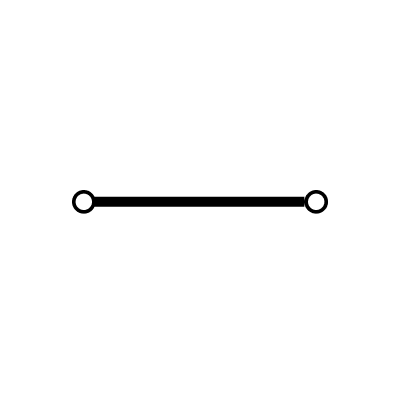
\includegraphics[width=\textwidth]{section3/3.2/open-interval.png}
		\caption{Open interval.}
	\end{subfigure}
	\hfill
	\begin{subfigure}[b]{0.2\textwidth}
		\centering
		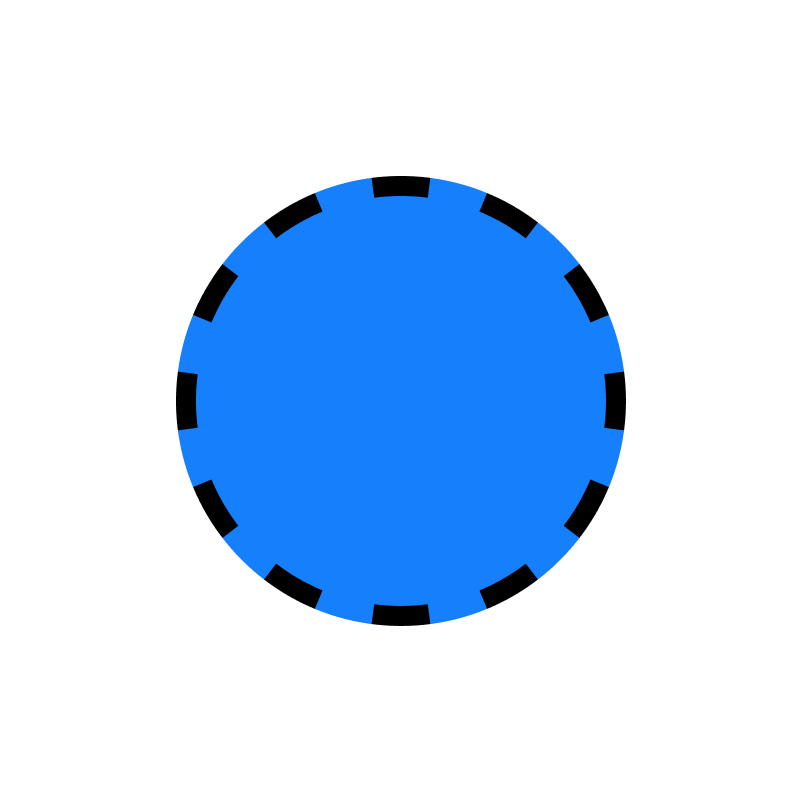
\includegraphics[width=\textwidth]{section3/3.2/open-disk.png}
		\caption{Open disk.}
	\end{subfigure}
	\hfill
	\begin{subfigure}[b]{0.2\textwidth}
		\centering
		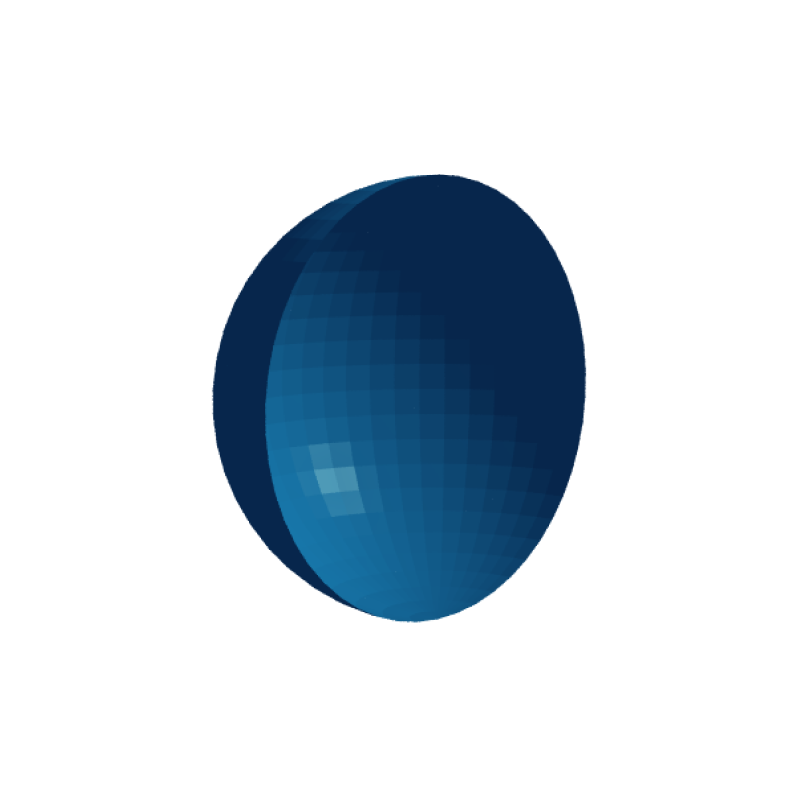
\includegraphics[width=\textwidth]{section3/3.2/open-sphere.png}
		\caption{Open "sphere".}
	\end{subfigure}
	\hfill
	\caption{Representation of different open sets varying in dimensional order.}
	\label{sec3.2:open-sets}
\end{figure}

   
    
\subsubsection{Closed Sets}
\begin{definition}[Closed Sets]
	A subset $X$ of a topological space $(W, T)$ is closed if its complement is open\footnote{This don't mean that closed sets are the opposite of open sets (e.g. the universe $W$ and the null set $\emptyset$ are both open and closed)\cite{mansfield_1987}.}. Closed sets hold the following properties which are duals of properties \eqref{ts:3.5} to \eqref{ts:3.7}. (Figure \ref{sec3.2:closed-sets})
				    
	\begin{property}
		The empty set $\emptyset$ and the universe $W$ are closed. \cite{mansfield_1987}
	\end{property}
	\begin{property}
		The intersection of a finite number of closed sets is a closed set. \cite{mansfield_1987}
	\end{property}
	\begin{property}
		The union of any collection of closed sets is a closed set. \cite{mansfield_1987}
	\end{property}
\end{definition}
    
\begin{figure}[ht]
	\centering
	\begin{subfigure}[b]{0.2\textwidth}
		\centering
		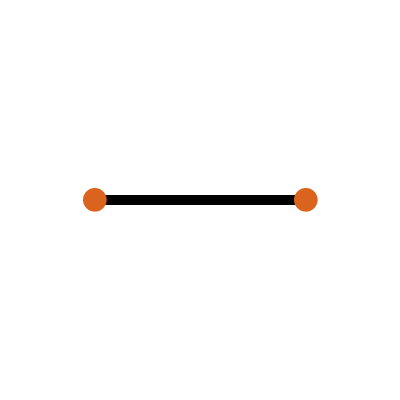
\includegraphics[width=\textwidth]{section3/3.2/closed-interval.png}
		\caption{Closed interval.}
	\end{subfigure}
	\hfill
	\begin{subfigure}[b]{0.2\textwidth}
		\centering
		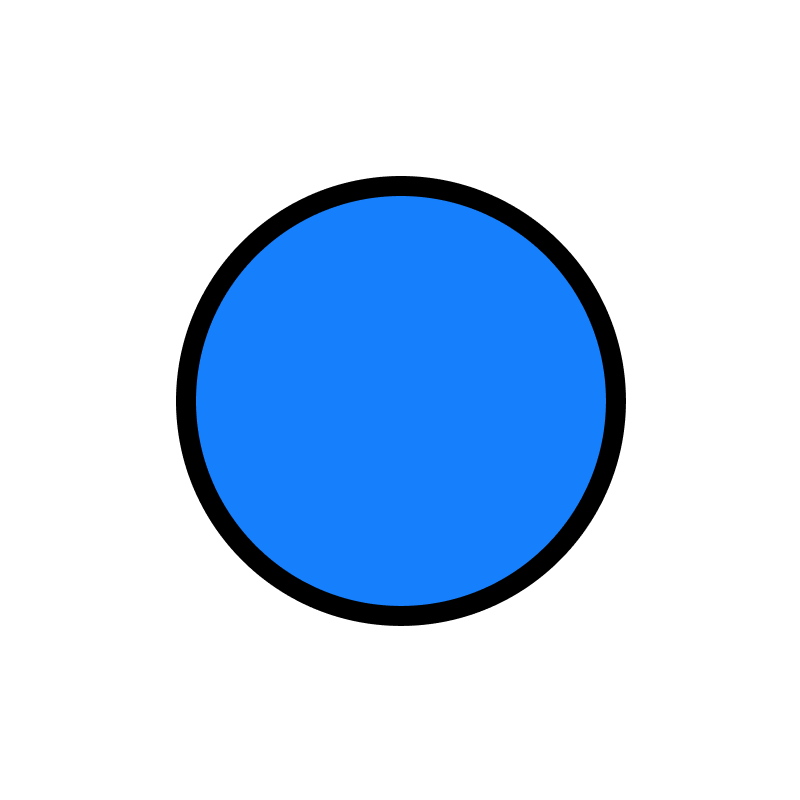
\includegraphics[width=\textwidth]{section3/3.2/closed-disk.png}
		\caption{Closed disk.}
	\end{subfigure}
	\hfill
	\begin{subfigure}[b]{0.2\textwidth}
		\centering
		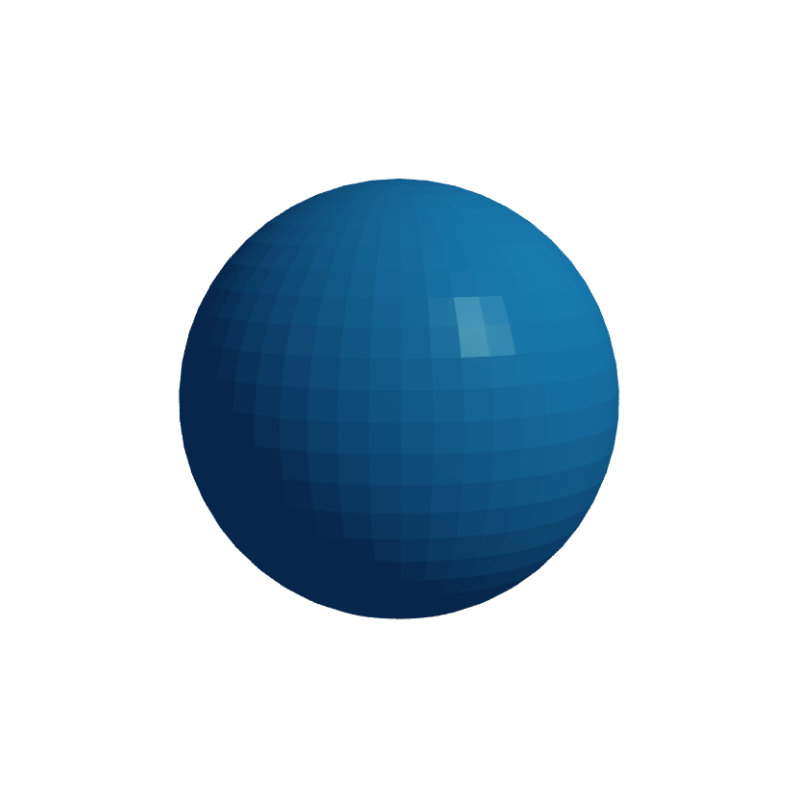
\includegraphics[width=\textwidth]{section3/3.2/closed-sphere.png}
		\caption{Closed sphere.}
	\end{subfigure}
	\hfill
	\caption{Representation of different closed sets varying in dimensional order.}
	\label{sec3.2:closed-sets}
\end{figure}

\subsubsection{Neighborhood}
     
\begin{definition}
	The neighborhood, denoted $N(y)$, of a point $y$ in a topological space $(W, T)$ is any subset of $W$ which contains an open set which contains $y$. If $N(y)$ is an open set, it is called an open neighborhood. \cite{Requicha1978MathematicalFO} (Figure \ref{sec3.2:interior-neighborhood})
\end{definition}
    
\subsubsection{Interior}
     
\begin{definition}
	A point of $y$ of $W$ is an interior point of a subset $X$ of $W$ if $X$ is a neighborhood of $y$. The interior of a subset $X$ of $W$, denoted $iX$, is the set of all the interior points of $X$.\cite{Requicha1978MathematicalFO} (Figure \ref{sec3.2:interior-neighborhood})
\end{definition}
    

\begin{figure}[ht]
	\begin{center}
		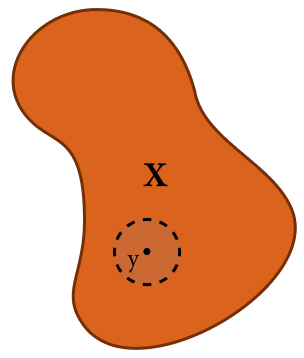
\includegraphics[width=0.2\textwidth]{section3/3.2/interior.png}
	\end{center}
	\caption{Interior point $y$ on a subset $X$. The disc around $y$ is the neighborhood of $y$.}
	\label{sec3.2:interior-neighborhood}
\end{figure}

\subsubsection{Boundary}
    
\begin{definition}
	A point $y$ of $W$ is a boundary point of a subset $X$ of $W$ if each neighborhood of $y$ intersects both $X$ and $cX$. The boundary of $X$, denoted $bX$, is the set of all boundary points of $X$. \cite{Requicha1978MathematicalFO} (Figure \ref{sec3.2:boundary})
\end{definition}
    
\begin{figure}[ht]
	\begin{center}
		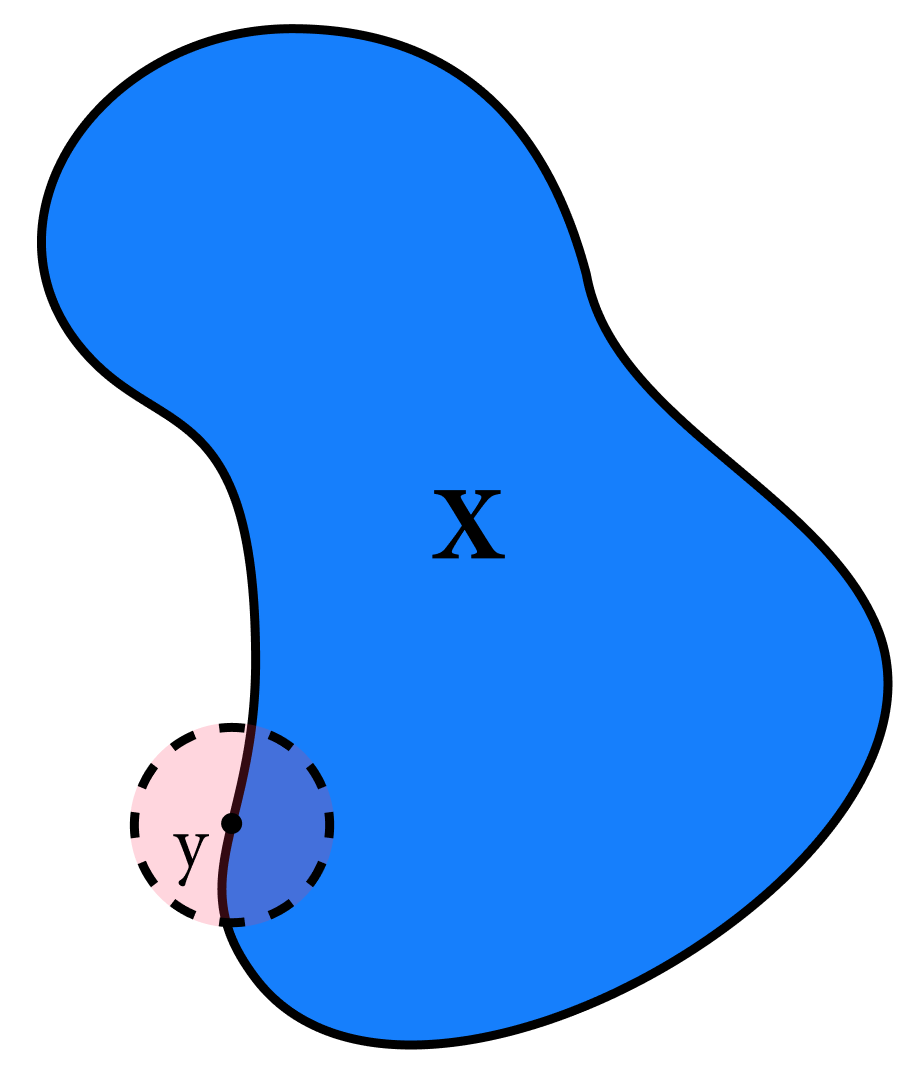
\includegraphics[width=0.2\textwidth]{section3/3.2/boundary.png}
	\end{center}
	\caption{Boundary point $y$ on a subset $X$.}
	\label{sec3.2:boundary}
\end{figure}
    
\subsubsection{Closure}
    
\begin{definition}
	The closure of a subset $X$, denoted $kX$, is the union of $X$ with the set of all its limit points. A point is a limit point of a subset $X$ of a topological space $(W, T)$ if each neighborhood of $y$ contains at least a point of $X$ different from $y$.  \cite{Requicha1978MathematicalFO} (Figure \ref{sec3.2:closure})
\end{definition}
    
\begin{figure}[ht]
	\begin{center}
		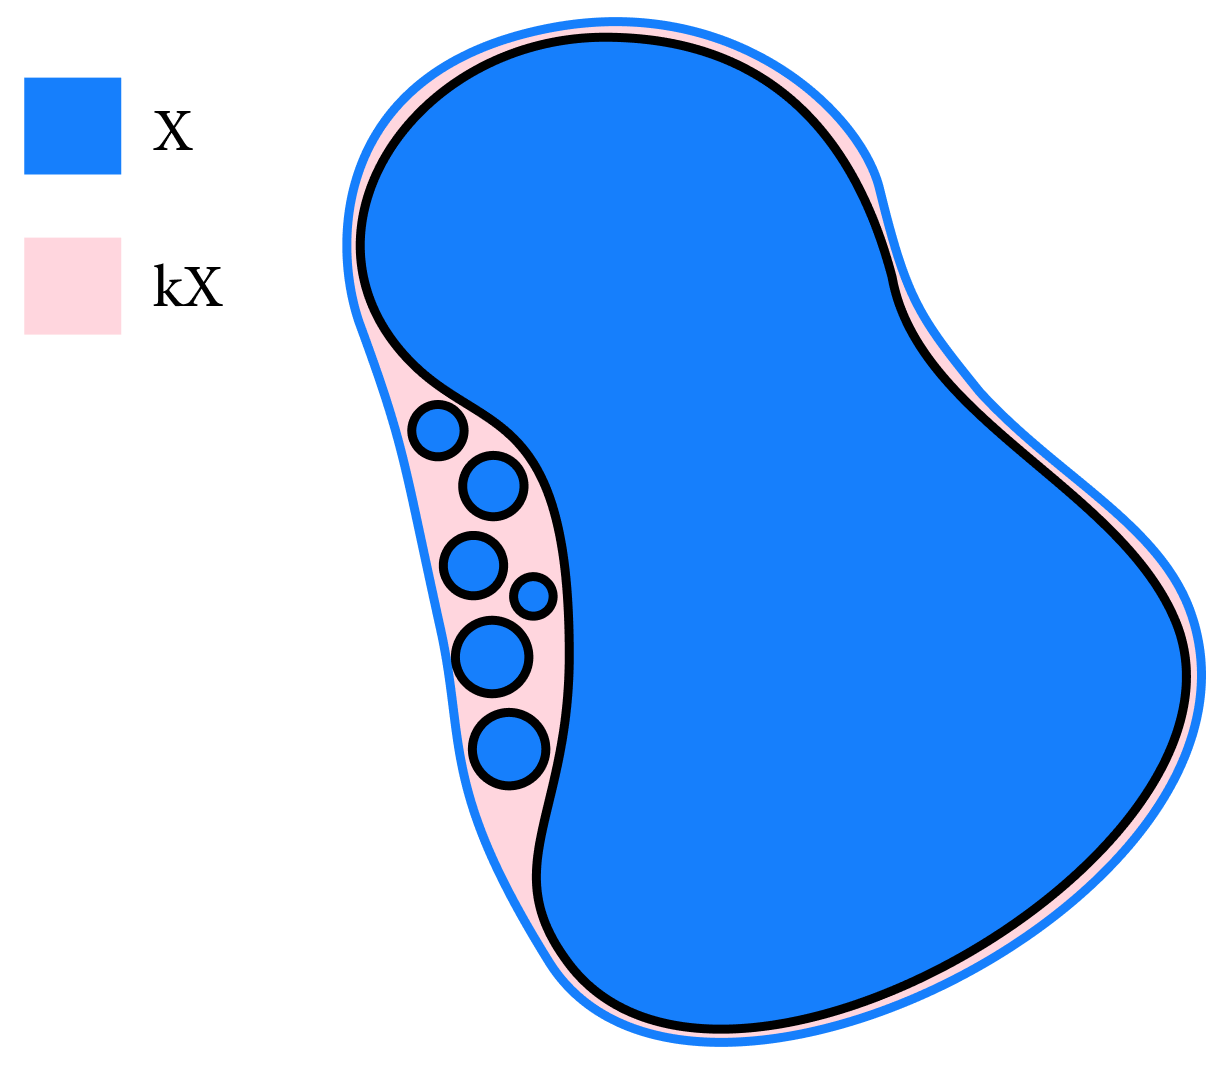
\includegraphics[width=0.3\textwidth]{section3/3.2/closure.png}
	\end{center}
	\caption{Closure $kX$ of a subset $X$.}
	\label{sec3.2:closure}
\end{figure}
    
\subsubsection{Regularity}
    
\begin{definition}[Regularity]
	The regularity of a subset $X$ of $W$, denoted $rX$, is the set of $rX = kiX$. \cite{mansfield_1987}
\end{definition}
\begin{definition}[Regular Set]
	A set $X$ is regular if $X = rX$, i.e. if $X = kiX$.  \cite{mansfield_1987} (Figure \ref{sec3.2:regularity}) 
\end{definition}
    
\begin{definition}[Regularized Set Operators]
	The regularized union, intersection, difference and complement are defined per:
	\begin{align*} 
		X \cup^* Y  & = r(X \cup Y)   \\
		X \cap^* Y  & = r(X \cap Y)   \\
		X \minus^*Y & = r(X \minus Y) \\
		c{^*}X      & = rcX           
	\end{align*}
\end{definition}
    
 
\begin{figure}[ht]
	\centering
	\begin{subfigure}[b]{0.3\textwidth}
		\centering
		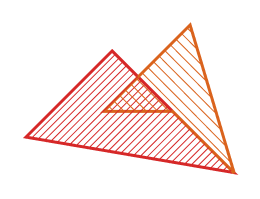
\includegraphics[width=\textwidth]{section3/3.2/regularization-initial.png}
		\caption{Initial polygons.}
		\label{sec3.2:initial-intersection}
	\end{subfigure}
	\hfill
	\begin{subfigure}[b]{0.3\textwidth}
		\centering
		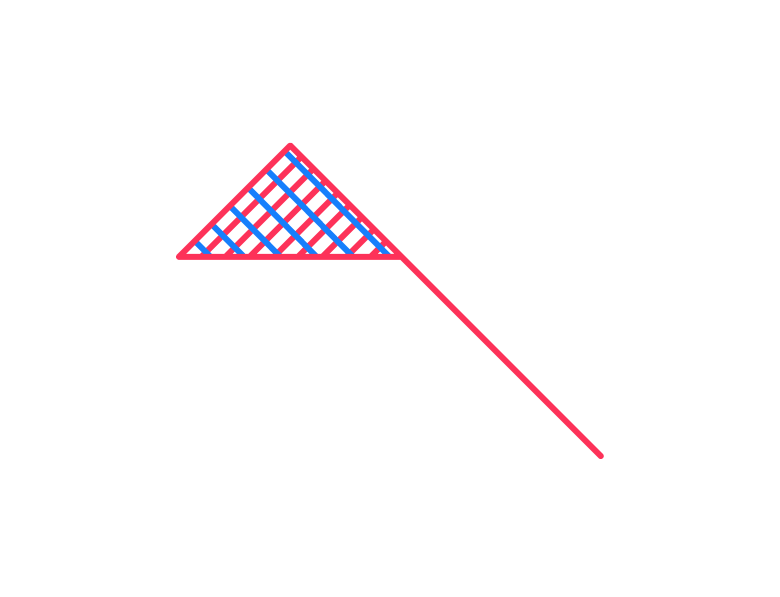
\includegraphics[width=\textwidth]{section3/3.2/regularization-non-regular.png}
		\caption{Typical intersection with dangling edge.}
		\label{sec3.2:normal-intersection}
	\end{subfigure}
	\hfill
	\begin{subfigure}[b]{0.3\textwidth}
		\centering
		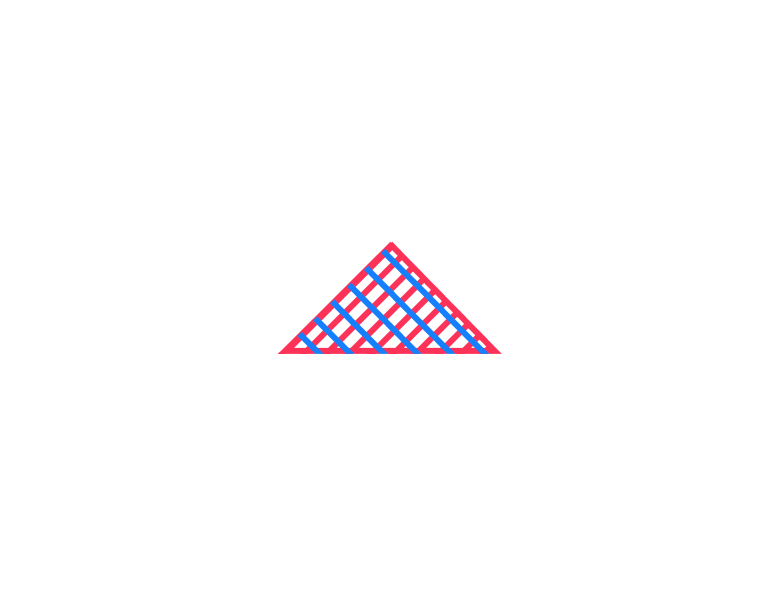
\includegraphics[width=\textwidth]{section3/3.2/regularization-regular.png}
		\caption{Regularized intersection.}
		\label{sec3.2:regular-intersection}
	\end{subfigure}
	\caption{Typical polygon intersection versus regularized intersection.}
	\label{sec3.2:regularity}
\end{figure}
   
\subsubsection{Membership Classification Function}
The membership classification function allows to segment a candidate set into three subsets which are the "inside", "outside", and "on the" of the reference set \cite{tilove1977a}. Here, we will abstractly define membership classification before moving to the practical implementations of the more specific ray classification.
This theory depends heavily on the previously defined notions of interior, closure, boundary, and regularity. For a brief recapitulation, a point $y$ is an element of the interior of a set $X$, denoted $iX$, if there exists a neighborhood of $y$ that is contained in $X$; $y$ is an element of the closure of $X$, $kX$, if every neighborhood of $y$ contains a point of $X$; $y$ is an element of the boundary of $X$, $bX$, if $y$ is an element of both $kX$ and $k(cX)$, where $c$ denotes the complement. A set is said to be regular if $X = kiX$.

The membership classification function works on a pair of point sets:

\begin{conditions}
	S     &  The regular reference set in a subspace $W$. \\
	X     &  The candidate regular set $X$, classified with respect to $S$, in a subspace $W'$ of $W$. \\
\end{conditions}

Primed symbols will be used	in order to denote operations on the subspace $W'$ while normal symbols will be used to denote the subspace $W$ (Table \ref{table:notations}).
 
\begin{table}
	\caption{Notation}
	\label{table:notations}
	\begin{tabularx}{\textwidth}{p{0.22\textwidth}X}
		\toprule
		$E^n$                                       & Euclidean $n$-space                                 \\
		$\emptyset$                                 & Empty Set                                           \\
		$W$                                         & Reference Set Universe                              \\
		$W'$                                        & Candidate Set Universe                              \\
		$\cup, \cap, \minus, c$                     & Set Operators                                       \\
		$\cup^*, \cap^*, \minus^*, c^*$             & Regularized Set Operators in $W$                    \\
		$\cup^{*'}, \cap^{*'}, \minus^{*'}, c^{*'}$ & Regularized Set Operators in $W'$                   \\
		$i, b, k, r$                                & interior, boundary, closure, and regularity in $W$  \\
		$i', b', k', r'$                            & interior, boundary, closure, and regularity in $W'$ \\
		\bottomrule
	\end{tabularx}
\end{table}

\begin{definition}
	The membership classification function, $M$ is defined as follows:
	\begin{equation}
		M[X, S] = (XinS, XonS, XoutS).
	\end{equation}
	where
	\begin{align*}
		XinS  & = X \cap^{*'} iS \\
		XonS  & = X \cap^{*'} bS \\
		XoutS & = X \cap^{*'} cS 
	\end{align*}
\end{definition}

The results obtained from this classification ($XinS, XonS, XoutS$) are the regular portions of the candidate set, $X$, in the interior, boundary, and the exterior of the reference set $W$ (Figure \ref{sec3.2:membership_classification}). The produced results are a quasi-disjoint decomposition of the candidate; therefore:
\begin{equation}
	X = XinS \cup XonS \cup XoutS
\end{equation}
and for "almost" all points in the subset:
\begin{align*}
	XinS \cap XonS  & = \emptyset \\
	XonS \cap XoutS & = \emptyset \\
	XinS \cap XoutS & = \emptyset \\
\end{align*}
We say almost since the subsets are generally not disjoint in the conventional sense. (e.g. in Figure \ref{sec3.2:membership_classification}, $XinS$ and $XonS$ share a boundary point). \cite{mansfield_1987}



\begin{figure}[ht]
	\begin{center}
		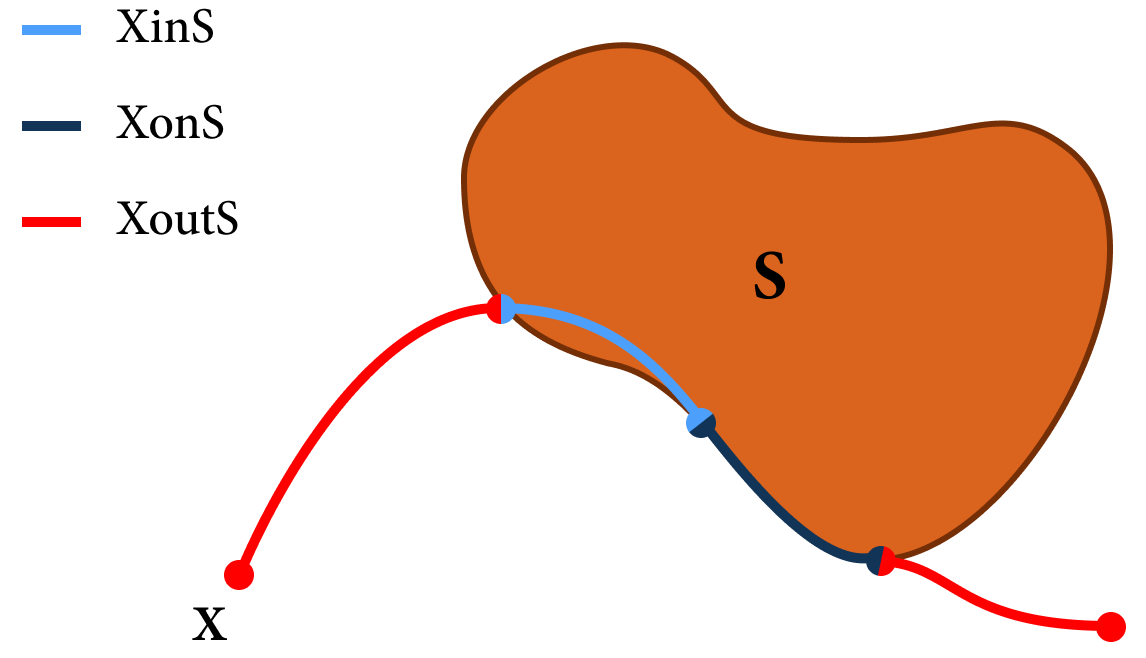
\includegraphics[width=0.5\textwidth]{section3/3.2/membership-classification.png}
	\end{center}
	\caption{Membership classification function.}
	\label{sec3.2:membership_classification}
\end{figure}

\subsubsection{Classification by constructive geometry}

Constructive geometry representations are binary trees whose nonterminal nodes designate regularized set operators and whose terminal nodes designate primitives.  We refer to the specific case of constructive geometry in $E^3$ where regularized compositions are constructed of solid primitives as constructive \textit{solid} geometry. Regular sets are closed under the regularized set operators thus a class of regular sets can be represented constructively as a combination of other more simple (regular) sets. \cite{Requicha1978MathematicalFO} 

For example, as illustrated in Figure \ref{sect3:halfplane-csg}, if the universe $W$ is in $E^2$ and we select the class of closed half-planes as our primitives, we could construct any regular set in $E^2$ given that it is bounded by a finite number of straight line segments.

\begin{figure}[ht]
	\begin{center}
		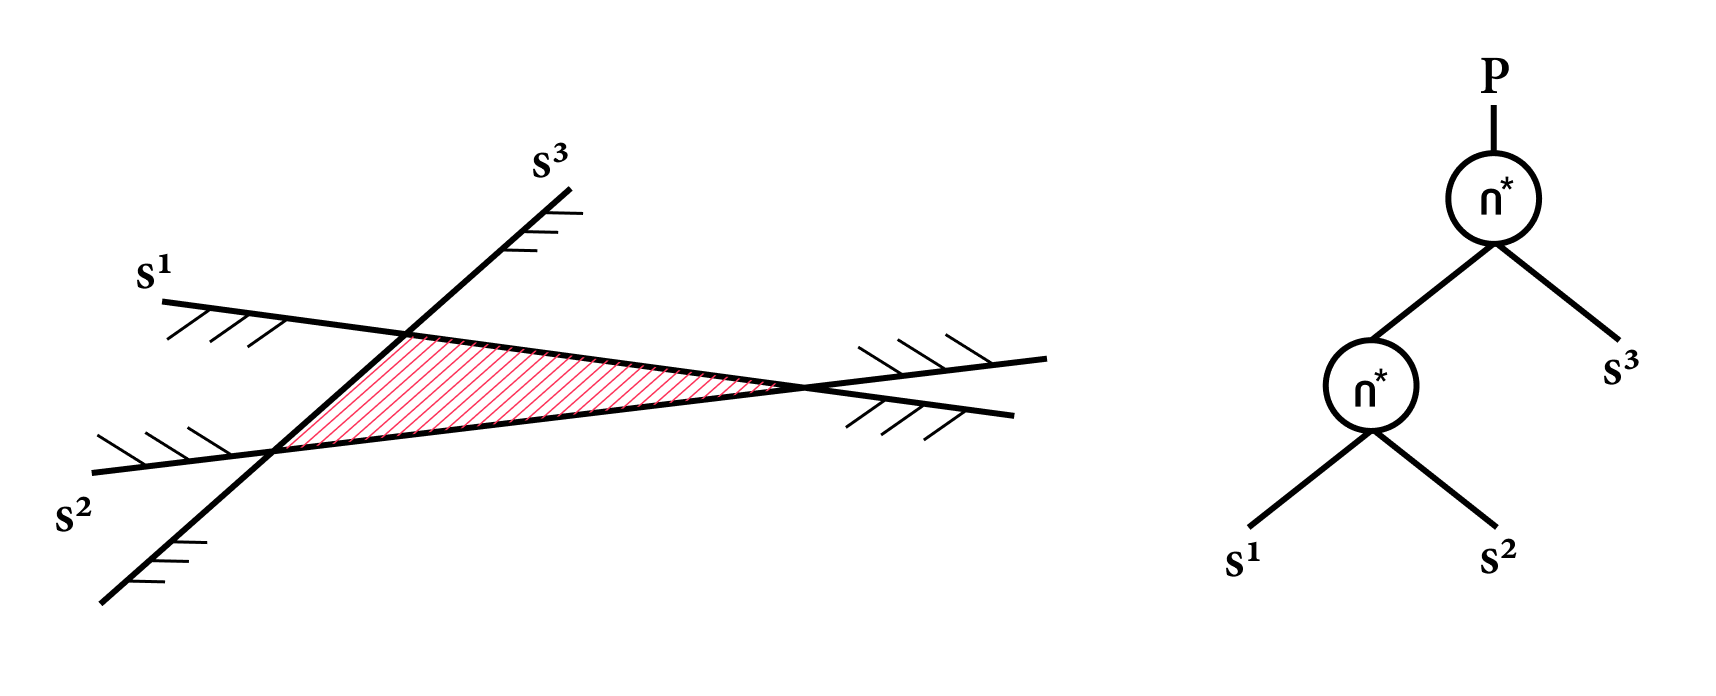
\includegraphics[width=0.8\textwidth]{section3/3.2/halfplane-csg.png}
	\end{center}
	\caption{A constructive representation of a polygon P using half-planes. The tree on the right is the constructive geometry representation.}
	\label{sect3:halfplane-csg}
\end{figure}

We choose to define the constructively represented regular sets using the divide-and-conquer paradigm as it is a natural approach to compute the value of such a function. Therefore, when a regular set $S$ is not a primitive, a nonterminal node, we convert the problem of evaluating the function $f(S)$ into two simpler instances of $f$ followed by a combine, $g$, step. When $S$ is a primitive, a terminal node, the problem can no longer be divided and an evaluator, $ef$, is used. We can now consider the general function for evaluation $M$ when the reference set $S$ is represented constructively.

\begin{align}
	M[X,S]= 
	\begin{cases}
	eM(X, S),                                                                & \text{if } S \subset A \\
	g(M[X, \text{l-subtree}(S)], M[X, \text{r-subtree}(S)], \text{root}(S)), & \text{otherwise}       
	\end{cases}
\end{align}

where

\begin{conditions}
	S     				  &  The regular reference set. \\
	X     				  &  The candidate regular set. \\
	eM     	  &  The primitive evaluation function. \\
	A     			  	  &  The set of all allowed primitives. \\
	g     				  &  The combine function. \\
	\text{l-subtree}     &  The left subtree. \\
	\text{r-subtree}     &  The right subtree. \\
	\text{root}     	  &  The operation type. \footnotemark \\
\end{conditions}
\footnotetext{The current node always contains the operation.}

To customize this general definition to be used in a specific domain, one must design the classification procedure, $eM$, and the combine procedure. We have partially defined our primitive classification procedure in Section \ref{section:ray-intersection}. The next section discusses both these procedures.

\subsection{Ray classification}
\label{sec3.3:ray-classification}

Given a ray and a solid composition tree, our procedure needs to classify the ray with respect to the solid and return the classification to the caller. As previously defined, the classification of a ray with respect to a solid is the information describing all ray-solid intersections. The procedure starts at the top of the solid composition tree, recursively descends to the terminal nodes, classifies the ray with respect to the primitives, then returns the array combining the classifications of the left and right subtrees. On the node level, this results in an array containing all possible intersections of a ray with the geometries in its left and right children. We must then sort each of these ray intersections by the distance to the ray origin and label them as inside or outside. We finally scan through this array and apply the boolean algebra rules in Table \ref{section3:boolean_algebra}. (See Figure \ref{sec3.3:classification}).
\begin{figure}[ht]
	\begin{center}
		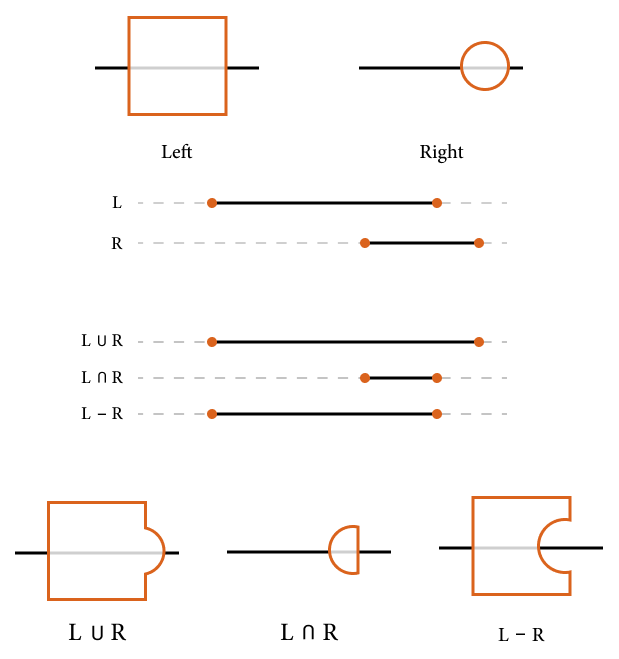
\includegraphics[width=0.8\textwidth]{section3/3.3/ray-classifications.png}
	\end{center}
	\caption{Example of combining ray classifications.}
	\label{sec3.3:classification}
\end{figure}

\begin{table}[H]
	\centering
	\caption{Boolean operations table}
	\label{section3:boolean_algebra}
	\begin{tabular}{||c c c c||} 
		\hline
		Set Operator & Left Solid & Right Solid & Composite \\ [0.5ex] 
		\hline\hline
		$\cup$       & $in$       & $in$        & $in$      \\
		             & $in$       & $out$       & $in$      \\
		             & $out$      & $int$       & $in$      \\
		             & $out$      & $out$       & $out$     \\
		             &            &             &           \\
		$\cap$       & $in$       & $in$        & $in$      \\
		             & $in$       & $out$       & $out$     \\
		             & $out$      & $in$        & $out$     \\
		             & $out$      & $out$       & $out$     \\
		             &            &             &           \\
		$\minus$     & $in$       & $in$        & $out$     \\
		             & $in$       & $out$       & $in$      \\
		             & $out$      & $in$        & $out$     \\
		             & $out$      & $out$       & $out$     \\		 	   	
		\hline
	\end{tabular}
\end{table}

\section{Optimization}

In this section, we will introduce the state-of-the-art CSG algorithm that is implemented in the OpenRT framework. Here we expose all the adjustments and changes we have made to the algorithm in order to maximize its performance and results. We will discuss a minimal hit classification algorithm, box enclosures, and how simple techniques such as "early-outs" can increase performance. Additionally, we propose the limitations of all these methods. Finally, we will put it all together in our version of the CSG algorithm.

\subsection{Minimal hit CSG classification}
\label{section:classification-optimization}


What we have introduced in the Section \ref{sec3.3:ray-classification} is the typical approach to rendering CSG. However, this approach could be very costly as we nest more geometries in the tree and require lots of memory to store, classify, and combine a long chain of operations and primitives. Additionally, the algorithm could also perform unnecessary checks when used in combination with BREPs. Therefore, we introduce a new approach which we refer to as minimal hit CSG classification. The approach described here computes intersections with binary CSG objects using the single nearest intersections whenever possible. Though a relatively similar algorithm has been introduced in \cite{kensler_ray_2006}, it was proven in \cite{csg-xrt-renderer} to not be functional for the intersection and difference operations. The following implementation addresses those issues and adds a few optimizations to the classification code. The general idea can be thought of as a simple finite state machine. First, we check for the closest intersections with both solids $A$ and $B$. We then classify those evaluations to three potential states: enter, exit, or miss. The enter and exit cases are checked using the same normal computation from before. The miss case is when the intersection distance remains to be the default value. Then depending on the operation, we evaluate the states and decide if we can already return one of them. If so, then we're done with the procedure. If not, we move the origin of the ray to the current viable intersection point and try the same over again. Figure \ref{sec4.1:fsm} illustrates the general idea behind the procedure.   

\begin{figure}[H]
	\centering
	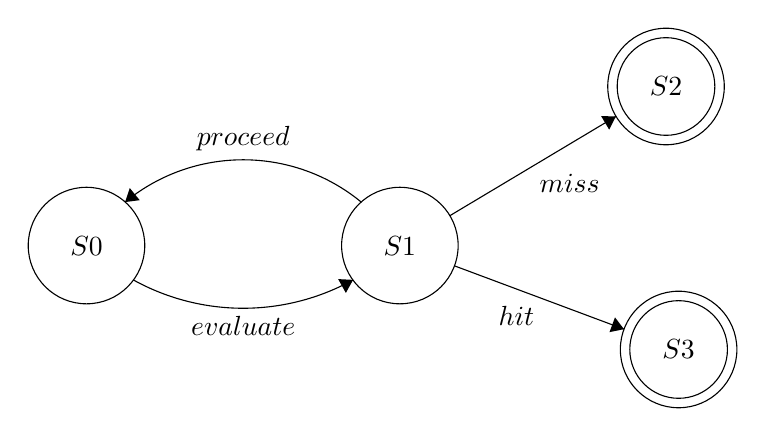
\begin{tikzpicture}[scale=0.2]
		\tikzstyle{every node}+=[inner sep=0pt]
		\draw [black] (40.8,-3.9) circle (3.7);
		\draw (40.8,-3.9) node {$S2$};
		\draw [black] (40.8,-3.9) circle (3.1);
		\draw [black] (41.6,-20.6) circle (3.7);
		\draw (41.6,-20.6) node {$S3$};
		\draw [black] (41.6,-20.6) circle (3.1);
		\draw [black] (4,-14) circle (3.7);
		\draw (4,-14) node {$S0$};
		\draw [black] (23.9,-14) circle (3.7);
		\draw (23.9,-14) node {$S1$};
		\draw [black] (6.445,-11.244) arc (129.44695:50.55305:11.811);
		\fill [black] (6.45,-11.24) -- (7.38,-11.12) -- (6.75,-10.35);
		\draw (13.95,-8.05) node [above] {$proceed$};
		\draw [black] (20.925,-16.183) arc (-61.07091:-118.92909:14.42);
		\fill [black] (20.93,-16.18) -- (19.98,-16.13) -- (20.47,-17.01);
		\draw (13.95,-18.48) node [below] {$evaluate$};
		\draw [black] (27.37,-15.29) -- (38.13,-19.31);
		\fill [black] (38.13,-19.31) -- (37.56,-18.56) -- (37.21,-19.5);
		\draw (31.3,-17.84) node [below] {$hit$};
		\draw [black] (27.08,-12.1) -- (37.62,-5.8);
		\fill [black] (37.62,-5.8) -- (36.68,-5.78) -- (37.19,-6.64);
		\draw (34.68,-9.45) node [below] {$miss$};
	\end{tikzpicture}
	\caption{Sample state diagram of the CSG procedure.}
	\label{sec4.1:fsm}
\end{figure}

There are a few sub-functions that we must also define in this case before introducing the general algorithm (Table \ref{table:procedure-details}).

\begin{table}
	\caption{Sub-procedures}
	\label{table:procedure-details}
	\begin{tabularx}{\textwidth}{p{0.30\textwidth}X}
		\toprule
		ReturnClosest        & Returns the closest of both.                                       \\
		ReturnFurthest       & Returns the furthest of both.                                      \\
		IfXCloserReturn      & Returns X if closer.                                               \\
		IfXFurtherReturn     & Returns X if further.                                              \\
		IfXCloserReturnFlip  & Returns X if closer and flips its normal.                          \\
		AdvanceToXLoop       & Sets the ray origin to intersection at X then loops.               \\
		AdvanceToClosestLoop & Sets the ray origin to the closest of both intersection then loops \\
		\bottomrule
	\end{tabularx}
\end{table}


\subsubsection{Union Classification}

Consider the case of two the spheres shown in Figure \ref{sec3.4:sphere-union}. The union of these two solids is the boundary of each of the spheres without their interior. Therefore, to find the correct classification results we must find the closest intersection from our ray origin such that it does not belong to the interior of the sphere.

\begin{figure}[ht]
	\centering
	\begin{subfigure}[b]{0.3\textwidth}
		\centering
		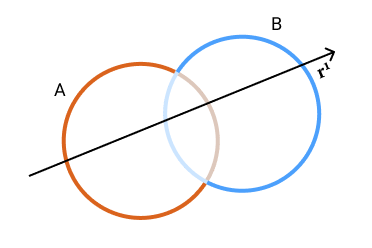
\includegraphics[width=\textwidth]{section4/4.1/union-case-1.png}
		\caption{Ray goes through both spheres.}
		\label{sec3.4:union-case1}
	\end{subfigure}
	\hfill
	\begin{subfigure}[b]{0.3\textwidth}
		\centering
		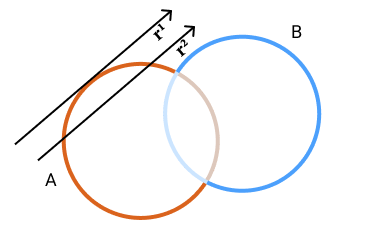
\includegraphics[width=\textwidth]{section4/4.1/union-case-2.png}
		\caption{Ray misses one of the spheres.}
		\label{sec3.4:union-case2}
	\end{subfigure}
	\hfill
	\begin{subfigure}[b]{0.3\textwidth}
		\centering
		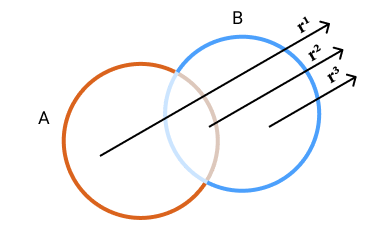
\includegraphics[width=\textwidth]{section4/4.1/union-case-3.png}
		\caption{Ray is inside one of the spheres.}
		\label{sec3.4:union-case3}
	\end{subfigure}
	\caption{Union ray classification cases.}
	\label{sec3.4:sphere-union}
\end{figure}

For the case where the ray enters both spheres (Figure \ref{sec3.4:union-case1}), our procedure would first get the closest intersections with A and B. Both these intersections would be classified as and enter; therefore, we must only find $MIN(A, B)$ in order to conclude which one of the boundaries of the sphere is closest.

Let us now examine the case where no intersection is found with one or all of the solids as shown in Figure \ref{sec3.4:union-case2}. If no intersection is found then both A and B's states are a miss and we return a miss. Otherwise, if only one of them is a miss then we return the other regardless if it's an enter or exit.

The last set of cases arise when the ray is shot from the interior of the spheres. This is more intricate since we have to teach our ray tracer to neglect the inner sides and only get the outer sides. If the first evaluation returns enter for B and exit for A, then we must check which one of them is closer. If A < B, then we return A. Otherwise, we move our origin to B and start the procedure again. If it is the opposite, then we perform the same logic but flip A with B. The final case is when the ray exits both A and B. Here, we return $MAX(A, B)$. Algorithm \ref{sec4.1:union-algo} shows the pseudocode for the union logic.

\begin{algorithm}[H]
	\SetAlgoLined
	\KwResult{Intersection Point}
	\While{true}{
		$min_A$ = intersectMin($A$)\;
		$min_B$ = intersectMin($B$)\;
		$state_A$ = classify($min_A$)\;
		$state_B$ = classify($min_B$)\;
		\uIf{$state_A$ == $miss$ \&\& $state_B$ == $miss$}{
			return $miss$\;
		}
		\uIf{$state_A$ == $miss$}{
			return $min_B$\;
		}
		\uIf{$state_B$ == $miss$}{
			return $min_B$\;
		}
		\uIf{$state_A$ == $state_B$}{
			\uIf{$state_A$ == $enter$}{
				ReturnClosest($min_A$, $min_B$)\;
			}
			\uIf{$state_A$ == $exit$}{
				ReturnFurthest($min_A$, $min_B$)\;
			}
		}
		\uIf{$state_A$ == $enter$ \&\& $state_B$ == $exit$}{
			IfXCloserReturn($min_B$)\;
			AdvanceToXLoop($min_A$)\;
		}
		\uIf{$state_A$ == $exit$ \&\& $state_B$ == $enter$}{
			IfXCloserReturn($min_A$)\;
			AdvanceToXLoop($min_B$)\;
		}
	}
	\caption{Minimal hit classification for union.}
	\label{sec4.1:union-algo}
\end{algorithm}

\subsubsection{Intersection Classification}

We will stick to the same general example; however, we will be performing the intersection of two spheres. (Figure \ref{sec3.4:sphere-intersection})

\begin{figure}[ht]
	\centering
	\begin{subfigure}[b]{0.3\textwidth}
		\centering
		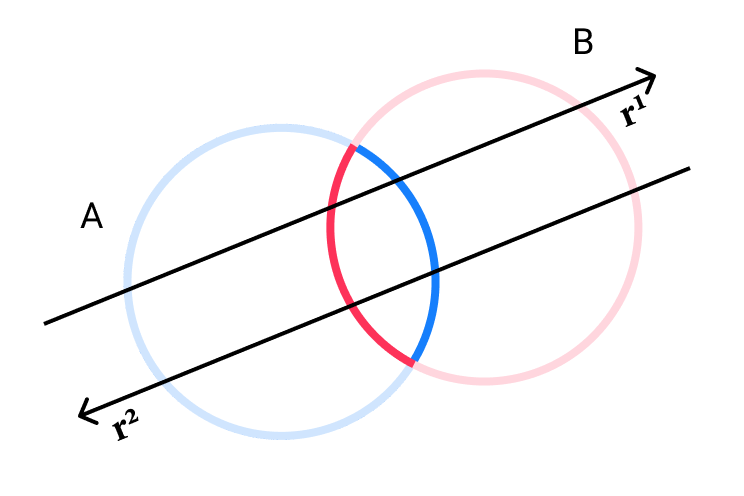
\includegraphics[width=\textwidth]{section4/4.1/intersection-case-1.png}
		\caption{Ray goes through both spheres.}
		\label{sec3.4:intersection-case-1}
	\end{subfigure}
	\hfill
	\begin{subfigure}[b]{0.3\textwidth}
		\centering
		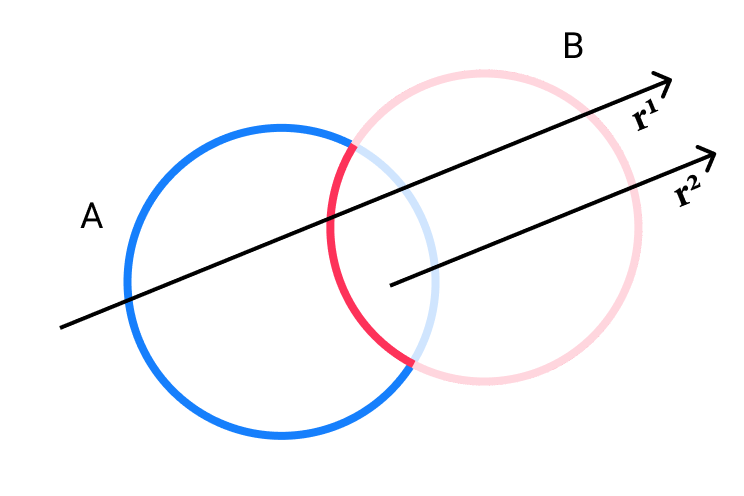
\includegraphics[width=\textwidth]{section4/4.1/intersection-case-2.png}
		\caption{Ray misses one of the spheres.}
		\label{sec3.4:intersection-case-2}
	\end{subfigure}
	\hfill
	\begin{subfigure}[b]{0.3\textwidth}
		\centering
		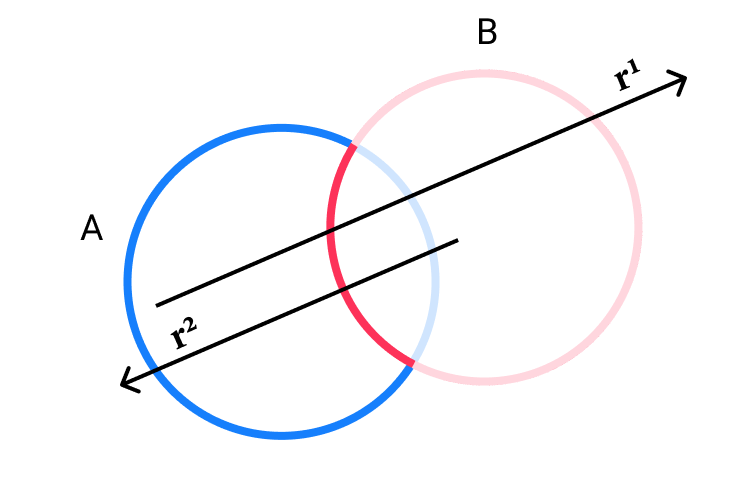
\includegraphics[width=\textwidth]{section4/4.1/intersection-case-3.png}
		\caption{Ray is inside one or both spheres.}
		\label{sec3.4:intersection-case-3}
	\end{subfigure}
	\caption{Intersection ray classification cases.}
	\label{sec3.4:sphere-intersection}
\end{figure}

The intersection of two spheres is their interior without the boundaries. We will apply the same previously defined notations shown in Table \ref{table:procedure-details}. First, we will begin with the obvious case where $A$ or $B$ classify as misses (Figure \ref{sec3.4:intersection-case-1}). By definition, the intersection is the shared area; therefore, if the ray misses one of the solids, we can already evaluate this as a $miss$.

The second case is when they both have the same classification. If both return an exit state, then we simply take the closest of both. However, if they both return an enter we either advance to A or B depending on which one is closest (Figure \ref{sec3.4:intersection-case-2}).

The final case is when the states are not a miss and also different to each other. If the A is an enter state while B is an exit state, then we return $A$ if its closer or move the ray origin to B and advance. We perform the opposite if A is exit and B is enter. Algorithm \ref{sec4.1:intersection-algo} shows the pseudocode for the intersection logic.

\begin{algorithm}
	\SetAlgoLined
	\KwResult{Intersection Point}
	\While{true}{
		$min_A$ = intersectMin($A$)\;
		$min_B$ = intersectMin($B$)\;
		$state_A$ = classify($min_A$)\;
		$state_B$ = classify($min_B$)\;
		\uIf{$state_A$ == $miss$ $||$ $state_B$ == $miss$}{
			return $miss$\;
		}
		\uIf{$state_A$ == $state_B$}{
			\uIf{$state_A$ == $enter$}{
				AdvanceToClosestLoop($min_A$, $min_B$)\;
			}
			\uIf{$state_A$ == $exit$}{
				ReturnClosest($min_A$, $min_B$)\;
			}
		}
		\uIf{$state_A$ == $enter$ \&\& $state_B$ == $exit$}{
			IfXCloserReturn($min_A$)\;
			AdvanceToXLoop($min_B$)\;
		}
		\uIf{$state_A$ == $exit$ \&\& $state_B$ == $enter$}{
			IfXCloserReturn($min_B$)\;
			AdvanceToXLoop($min_A$)\;
		}
	}
	\caption{Minimal hit classification for the intersection.}
	\label{sec3.4:intersection_algo}
\end{algorithm}

\subsubsection{Difference Classification}
\label{section:minimal_difference_classficiation}

The difference operations are not commutative nor distributive; therefore, the direction of the ray renders completely different results. We shall stick to the same example as the previous two cases and with similar notations (Figure \ref{sec3.4:sphere-difference}).

\begin{figure}[ht]
	\centering
	\begin{subfigure}[b]{0.3\textwidth}
		\centering
		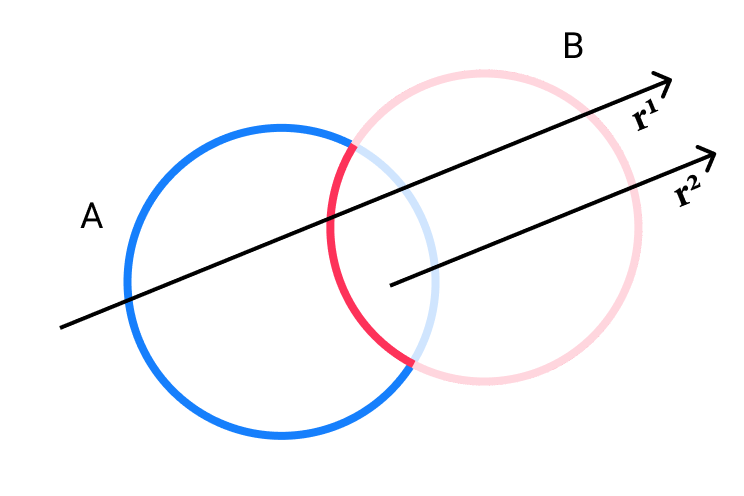
\includegraphics[width=\textwidth]{section4/4.1/difference-case-2.png}
		\caption{Ray misses one of the spheres.}
		\label{sec3.4:difference-case-1}
	\end{subfigure}
	\hfill
	\begin{subfigure}[b]{0.3\textwidth}
		\centering
		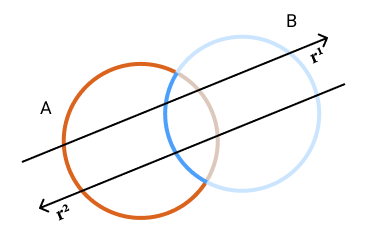
\includegraphics[width=\textwidth]{section4/4.1/difference-case-1.png}
		\caption{Ray goes through both spheres.}
		\label{sec3.4:difference-case-2}
	\end{subfigure}
	\hfill
	\begin{subfigure}[b]{0.3\textwidth}
		\centering
		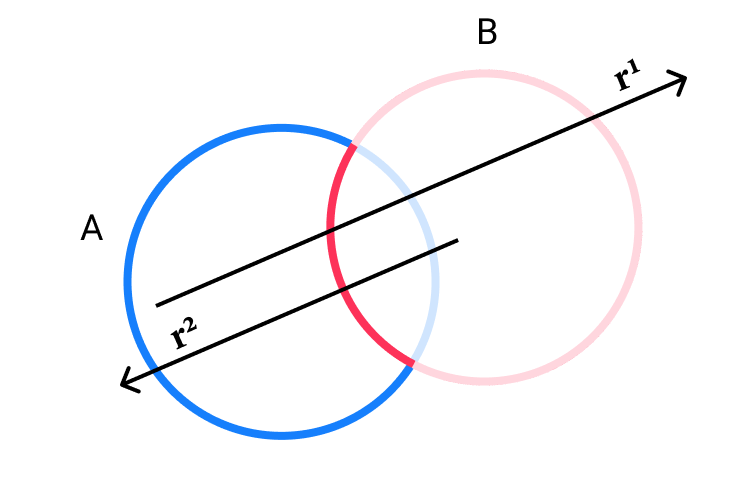
\includegraphics[width=\textwidth]{section4/4.1/difference-case-3.png}
		\caption{Ray is inside one or both spheres.}
		\label{sec3.4:difference-case-3}
	\end{subfigure}
	\caption{Difference ray classification cases.}
	\label{sec3.4:sphere-difference}
\end{figure}


We will first consider the case where a ray misses one of the two spheres, as shown in Figure \ref{sec3.4:difference-case-1}. If the ray only misses A or both, then we consider this a miss. If the ray only misses B, we return A regardless of enter or exit.

The second case is when they both have the same classification. If both return an exit state, then we return B if closer and flip the normal. Otherwise, we advance the ray origin to B. However, if they both return an enter we return A if it's closer or advance to the hit point of B.

The last and most complicated case is when the classifications are different to each other. If the ray enters A and exits B, we return B if it's closer or advance to A. However, if the classifications are the opposite, we advance to whichever is closer and continue. Algorithm \ref{sec4.1:difference-algo} shows the pseudocode for the difference logic.

\begin{algorithm}[H]
	\SetAlgoLined
	\KwResult{Intersection Point}
	\While{true}{
		$min_A$ = intersectMin($A$)\;
		$min_B$ = intersectMin($B$)\;
		$state_A$ = classify($min_A$)\;
		$state_B$ = classify($min_B$)\;
		\uIf{$state_A$ == $miss$}{
			return $miss$\;
		}
		\uIf{$state_B$ == $miss$}{
			return $min_A$\;
		}
		\uIf{$state_A$ == $enter$ \&\& $state_B$ == $enter$}{
			IfXCloserReturn($min_A$)\;
			AdvanceToXLoop($min_B$)\;
		}
		\uIf{$state_A$ == $exit$ \&\& $state_B$ == $exit$}{
			IfXCloserReturnFlip($min_B$)\;
			AdvanceToXLoop($min_A$)\;
		}
		\uIf{$state_A$ == $enter$ \&\& $state_B$ == $exit$}{
			AdvanceToClosestLoop($min_A$, $min_B$)\;
		}
		\uIf{$state_A$ == $exit$ \&\& $state_B$ == $enter$}{
			IfXCloserReturnFlip($min_A$)\;
			return $min_B$
		}
	}
	\caption{Minimal hit classification for the difference.}
	\label{sec3.4:difference_algo}
\end{algorithm} 


\subsection{Bounding Boxes}
\label{section:bounding-boxes-optimization}

Bounding boxes are the simplest way to cut down on the number of ray intersection operations and reduce overall rendering time \cite{efficient_csg_meshes}. Let us imagine the situation where a union of two spheres composed of 100 triangles lies in the middle of a 500x500px view of which the composite covers 100x100 pixels. In the former approach, we would examine every single ray with the complete composite. Resulting in a staggering $25.000.000$ intersection checks; though,  we solely necessitate a fifth of that. We introduce a box enclosure to do a preliminary examination before testing the rest of the composite. Hence, with a tight enough box (covering 110x110), the ray tracer would only need to check for $1.460.000$ intersections such that $250.000$ tests are box enclosure ones and the rest $1.210.000$ are ray-solid tests - a decrease of roughly $80\%$. In the worst case, when an enclosure stretches across the entire view, the box enclosure will add additional operations of ray-box intersections on top of completing all the ray-intersection checks. Nevertheless, ray-box tests are fast, and one could dismiss the additional costs of those operations. When this method is used in the context of CSG, this solution essentially turns into an efficient binary tree traversal \cite{ROTH1982109}. 

We can also use many other types of enclosures; however, we choose box enclosures for their numerous advantages. First, one can define an abstract box by only two points (a minimum and maximum point). Because the enclosure definition lies inside every node in the CSG tree, we must ensure that we do not excessively increase the required memory per node. Second, boxes are arguably the tightest types of bounding volumes. Implying that if a ray-box intersection test is positive, there is a high probability the ray will too intersect the geometry inside of the bounding box. Lastly, applying boolean operations on bounding boxes is straightforward. Therefore, if an object is part of a CSG tree, but the precomputed bounding box is smaller than the object (e.g., the case of a subtraction operation), the rest of the geometry piercing outward will also be neglected when performing ray-composite intersection tests \cite{ROTH1982109}.

A bounding box is a rectangular parallelepiped defined by exactly two points (Figure \ref{sec4.2:box-points}). Each primitive, solid, and composite must be able to define its bounding box. For primitive cases, the bounding box is case-specific. For example, the bounding box of a primitive sphere of radius $r = 1$ located at center point $\vec{o} = (0, 0, 0)$ has a bounding box whose maximum point is $(r, r, r)$ and minimum point $(-r, -r, -r)$. Solids are more complicated as they are composed of many primitives. Hence, one has to create a collapsed bounding box (a bounding box whose $min$ and $max$ coordinates are respectively $+\inf$ and $-\inf$) and slowly start inflating by the primitive's predefined boxes. The inflation step is as simple as checking if the value of a coordinate of the current bounding box is smaller or bigger than that of the primitive's bounding box and either picking the smallest or the greatest value depending on the point being checked. For instance, if our current bounding box has $min(0, 0, 0)$ and $max(1, 1, 3)$ and the current primitives bounding box has $min2(-1, -1, 1)$ and $max2(2, 2, 2)$ then the current values of the points of the inflated bounding box become $min(-1, -1, 0)$ and $max(2, 2, 3)$.


\begin{figure}[ht]
	\begin{center}
		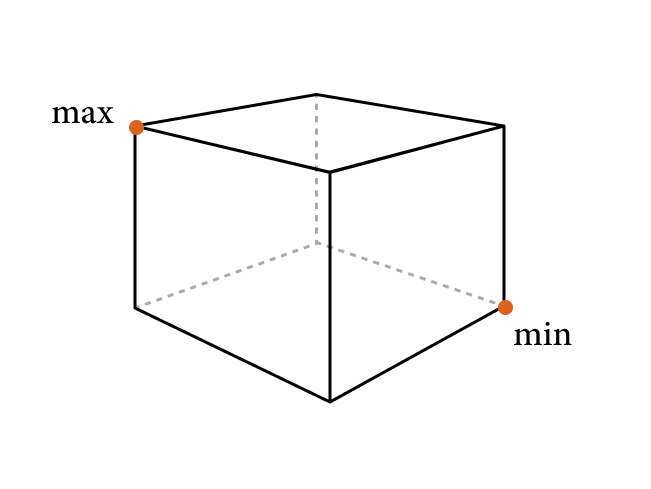
\includegraphics[width=0.5\textwidth]{section4/4.2/box-enclosure-points.png}
	\end{center}
	\caption{Bounding box.}
	\label{sec4.2:box-points}
\end{figure}

Combining the boxes on the composite level is also very important to realize. We can achieve this trivially with the usual rules of algebra defined in the previous section. Though that doesn't hold for the difference operation as its results are not trivially foreseeable, and the cost of analyzing the entire composition is counter-productive in this case \cite{ROTH1982109}. When dealing with the union operation, we select the smallest value from both boxes per coordinate for the minimum and vice-versa. For the intersection operation, we pick the highest value from both boxes per coordinate for the minimum - opposite to the union.
The dual for the maximum.  For the difference, we have previously mentioned that it's not possible to generalize using boolean algebra; therefore, we keep the minimum and maximum of the left box as we are sure that the result of the subtraction operation will never be bigger than the left geometry, $A - B \leq A$. Figure \ref{sec4.2:composite-bounding-box} shows the different operations on rectangles. The same logic holds for the three-dimensional solids as we only check for an additional coordinate. Algorithm \ref{sec4.2:composite-box} defines the procedure for composite boxes \cite{ROTH1982109}.

\begin{figure}[ht]
	\centering
	\begin{subfigure}[b]{0.4\textwidth}
		\centering
		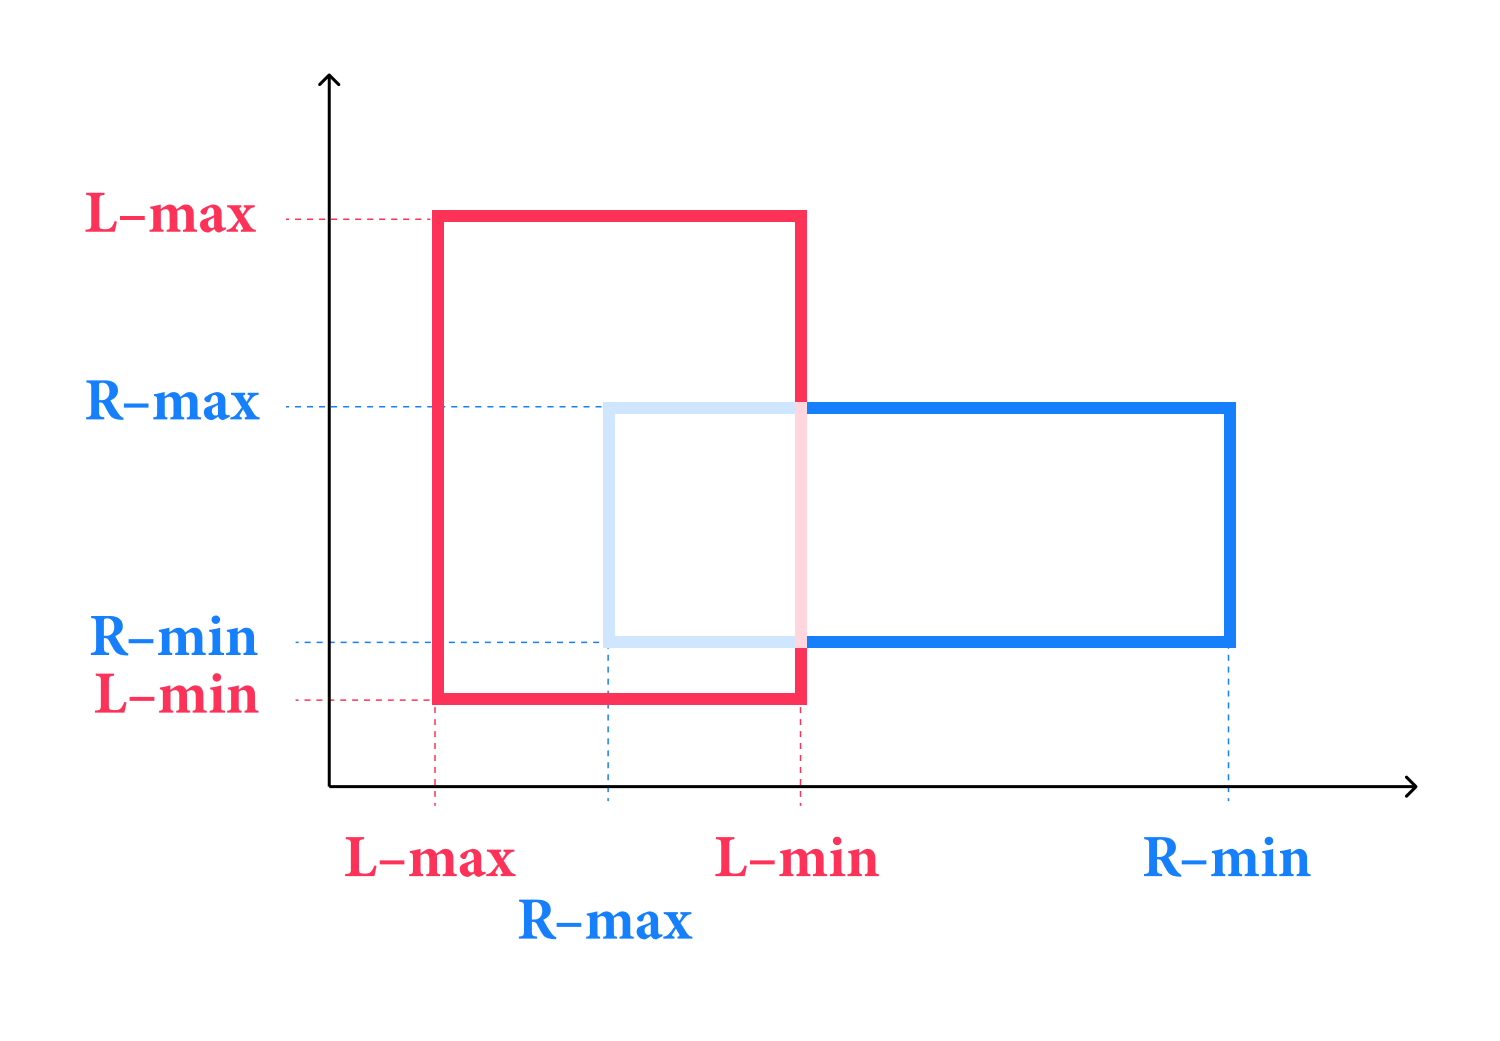
\includegraphics[width=\linewidth]{section4/4.2/box-enclosure-initial.png}
		\caption{Initial bounding boxes.}
		\label{sec4.2:composite-box-base}
	\end{subfigure}
	\hfill
	\begin{subfigure}[b]{0.4\textwidth}
		\centering
		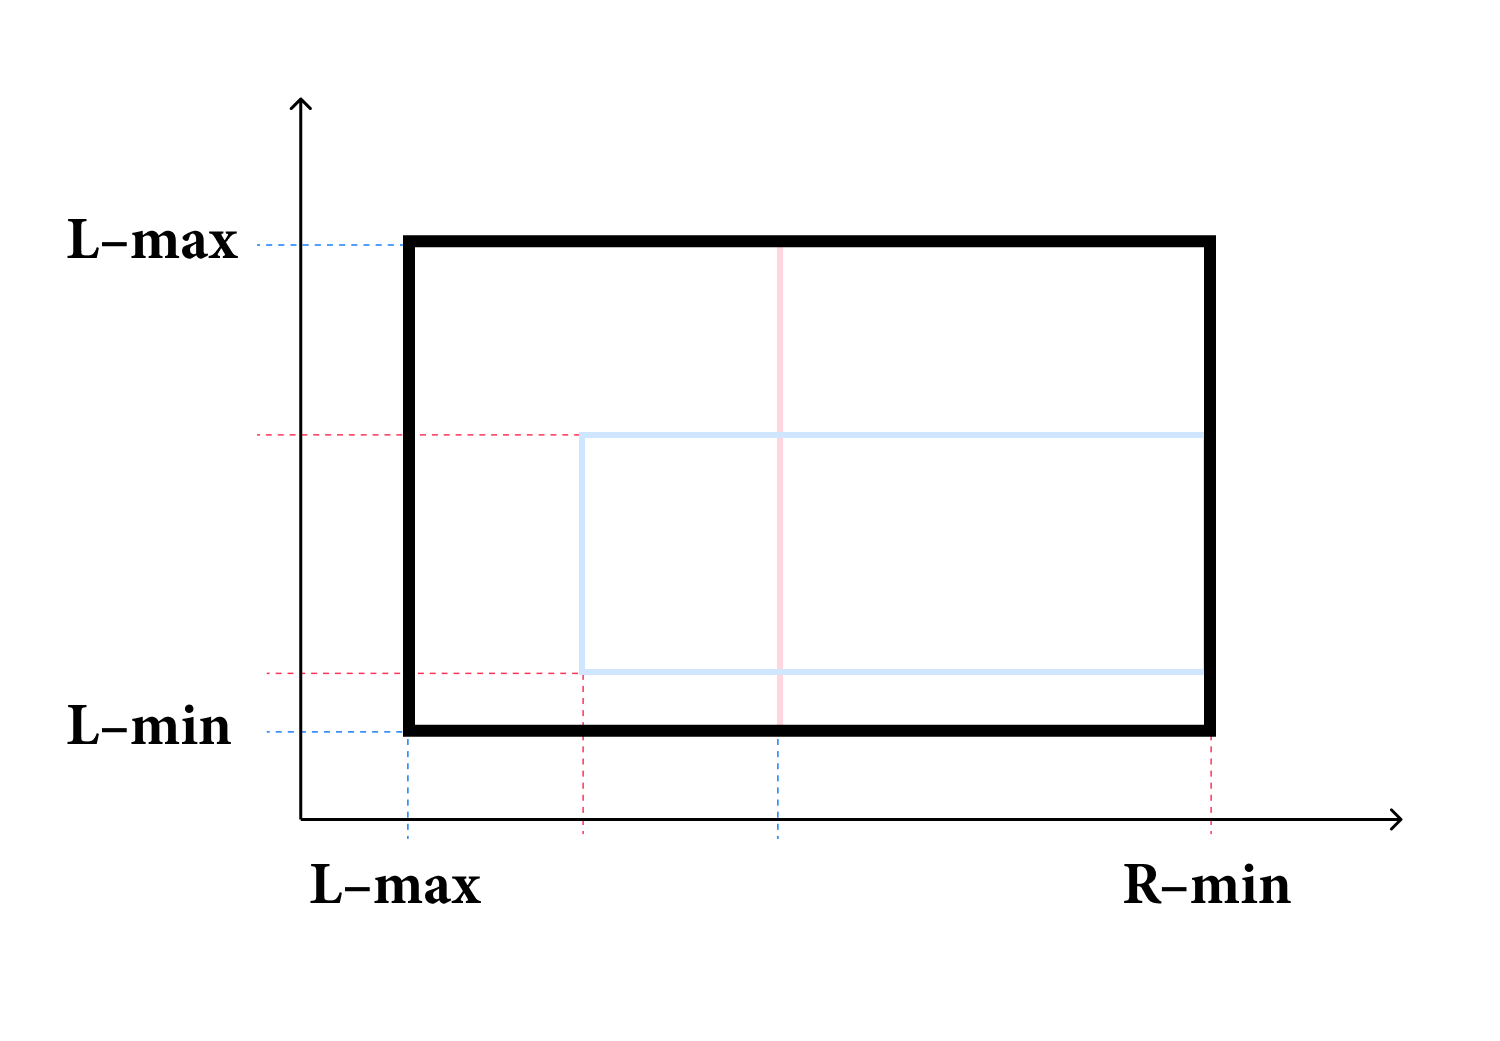
\includegraphics[width=\linewidth]{section4/4.2/box-enclosure-union.png}
		\caption{Union of bounding boxes.}
		\label{sec4.2:composite-box-union}
	\end{subfigure}
	\medskip
	\begin{subfigure}[b]{0.4\textwidth}
		\centering
		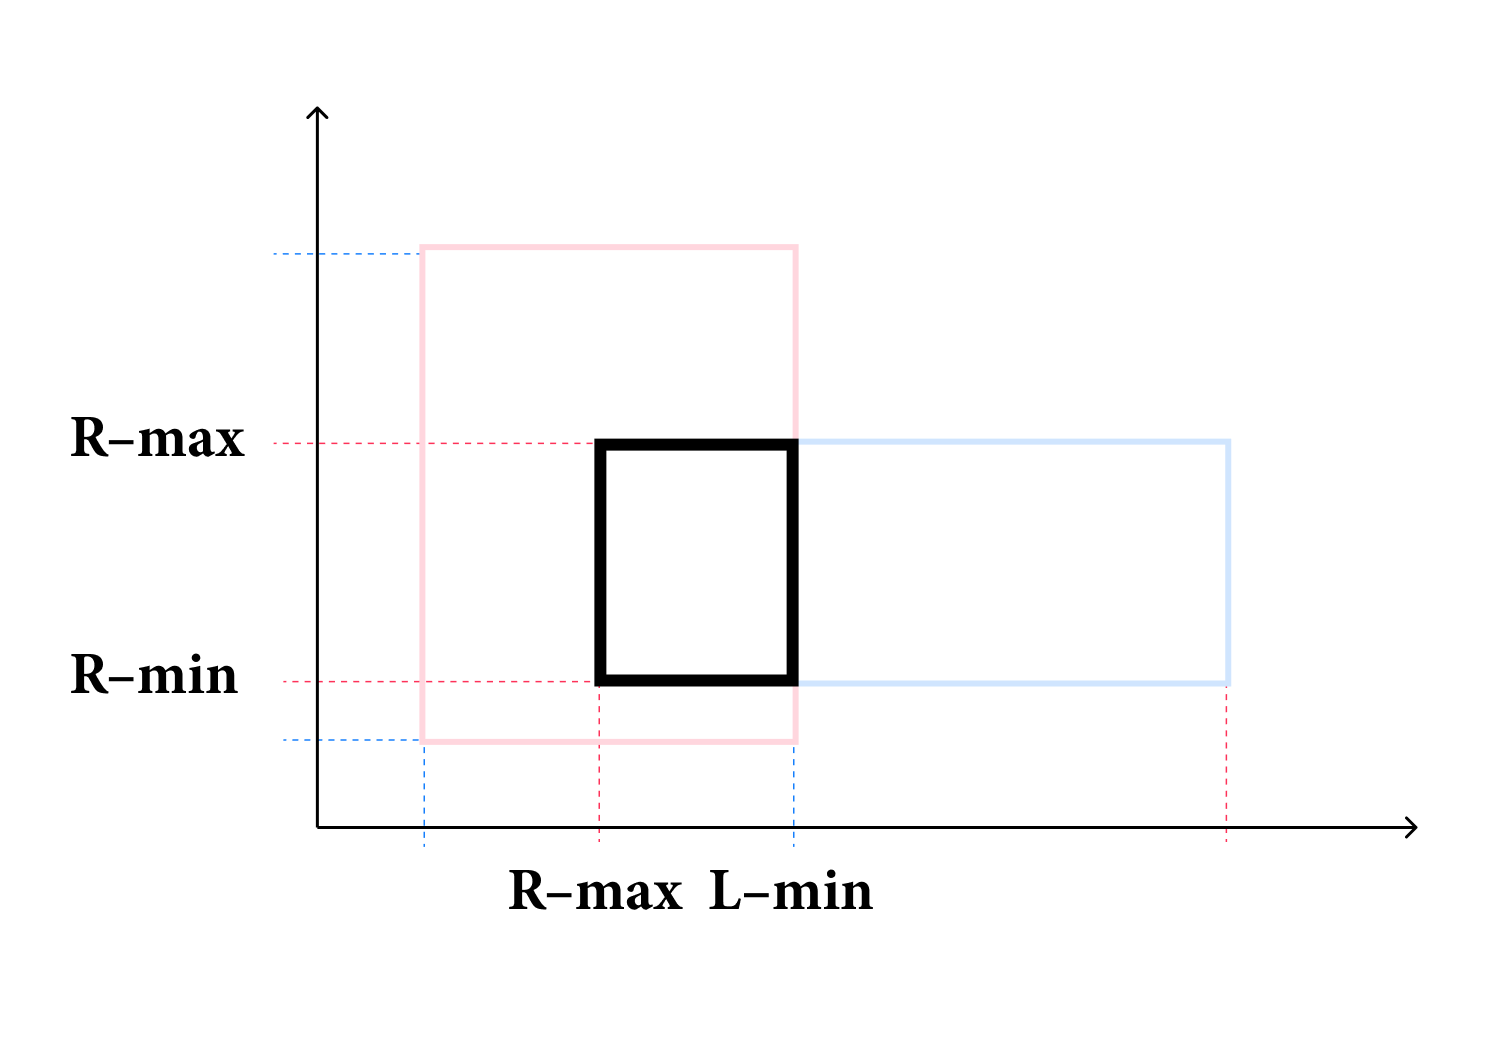
\includegraphics[width=\linewidth]{section4/4.2/box-enclosure-intersection.png}
		\caption{Intersection of bounding boxes.}
		\label{sec4.2:composite-box-intersection}
	\end{subfigure}
	\hfill
	\begin{subfigure}[b]{0.4\textwidth}
		\centering
		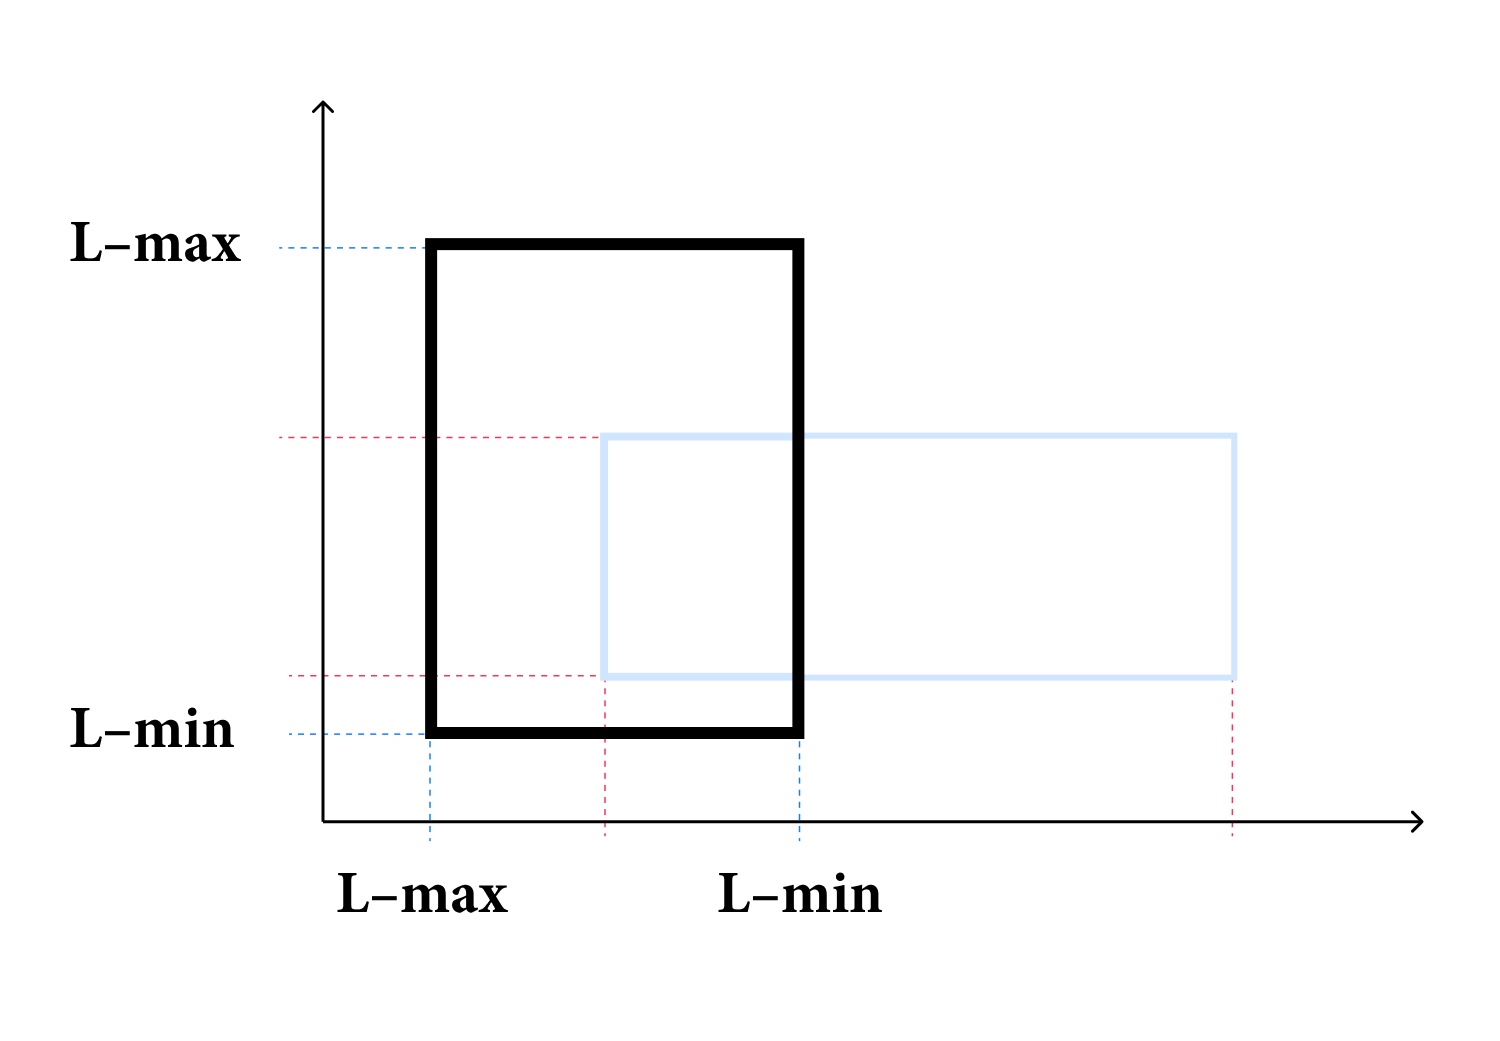
\includegraphics[width=\linewidth]{section4/4.2/box-enclosure-difference.png}
		\caption{Difference of bounding boxes.}
		\label{sec4.2:composite-box-difference}
	\end{subfigure}
	\caption{Composite bounding boxes.}
	\label{sec4.2:composite-bounding-box}
\end{figure}

\begin{algorithm}[H]
	\SetAlgoLined
	\KwResult{Composite bounding box}
	\For{$i$ = 1, 2, 3}{
		\uIf{Operator is $\cup$}{
			min[$i$] = MIN(leftMin[$i$], rightMin[$i$])\;
			max[$i$] = MAX(leftMax[$i$], rightMax[$i$])\;
		}
		\uIf{Operator is $\cap$}{
			min[$i$] = MAX(leftMin[$i$], rightMin[$i$])\;
			max[$i$] = MIN(leftMax[$i$], rightMax[$i$])\;
		}
		\uIf{Operator is $\minus$}{
			min[$i$] = leftMin[$i$]\;
			max[$i$] = leftMax[$i$]\;
		}
	}
	\caption{Composite solid box enclosure estimation algorithm.}
	\label{sec4.2:composite-box}
\end{algorithm} 

\subsection{Binary Space Partitioning Trees}
\label{section:bsp-optimization}

One of the most fundamental concepts in ray tracing is spatial or hierarchical data structures built using binary space subdivision to efficiently search for objects in the scene \cite{ray_tracing_BSP2}. A predominant concept in these data structures is binary space partitioning which refers to the successive subdivision of a scene's bounding box with planes until we reach termination criteria. The resulting data structure is called a binary space partition tree or a BSP tree. BSP trees offer the flexibility of using arbitrarily oriented planes to accommodate complex scenes and uneven spatial distributions. Therefore, in theory, BSP trees are a simple, elegant, and efficient solution to our visible-surface problems. In our implementation, we use a variant called KD-trees - which we refer to as BSP here. These are a more "restricted" type of BSP trees in which only axis-aligned splitting planes are allowed. These trees conform much better with computational advantages and memory needs but do not adapt very well to scene complexities. It is relatively easy to generate an inefficient binary tree with non-axis-aligned geometry (e.g., a long skinny cylinder oriented diagonally) \cite{ray_tracing_BSP}. All variations of the algorithms are generally composed of two fundamental parts, building and traversing the tree. How we choose these two core procedures tremendously affects the amount of acceleration achievable. We will discuss our building and traversing procedures. Because the main focus of the work doesn't align with the improvement of building or traversal procedures, the BSP algorithm is unoptimized. However, many algorithms such as surface area heuristic, local greedy SAH, automatic termination criteria, and many more have proved to optimize KD trees \cite{fast_building_kd_trees, parallel_kd_tree_construction}.

\subsubsection{Building BSP trees}

The tree is constructed recursively in a top-down manner, making a local greedy decision about the splitting planes. We use axis-aligned bounding boxes to wrap the nodes. We choose the split dimension using the current largest dimension (i.e., if the box is biggest in its $x$ axis then we will pick that as our splitting plane.). We then position the plane is positioned at the spatial median of the dimension. The subdivision is performed until either the number of primitives in a single node falls below a predefined threshold or the tree depth exceeds a maximum value.  The user provides these stopping criteria. To better illustrate the algorithm, we will utilize the simple two-dimensional KD-tree and the triangles in Figure \ref{sec4.3:example-kd-tree}. Each node in the tree represents a triangle, and each internal node represents an axis-aligned rectangular region with an axis-aligned plane that separates the regions of its two children.

\begin{figure}[ht]
	\begin{center}
		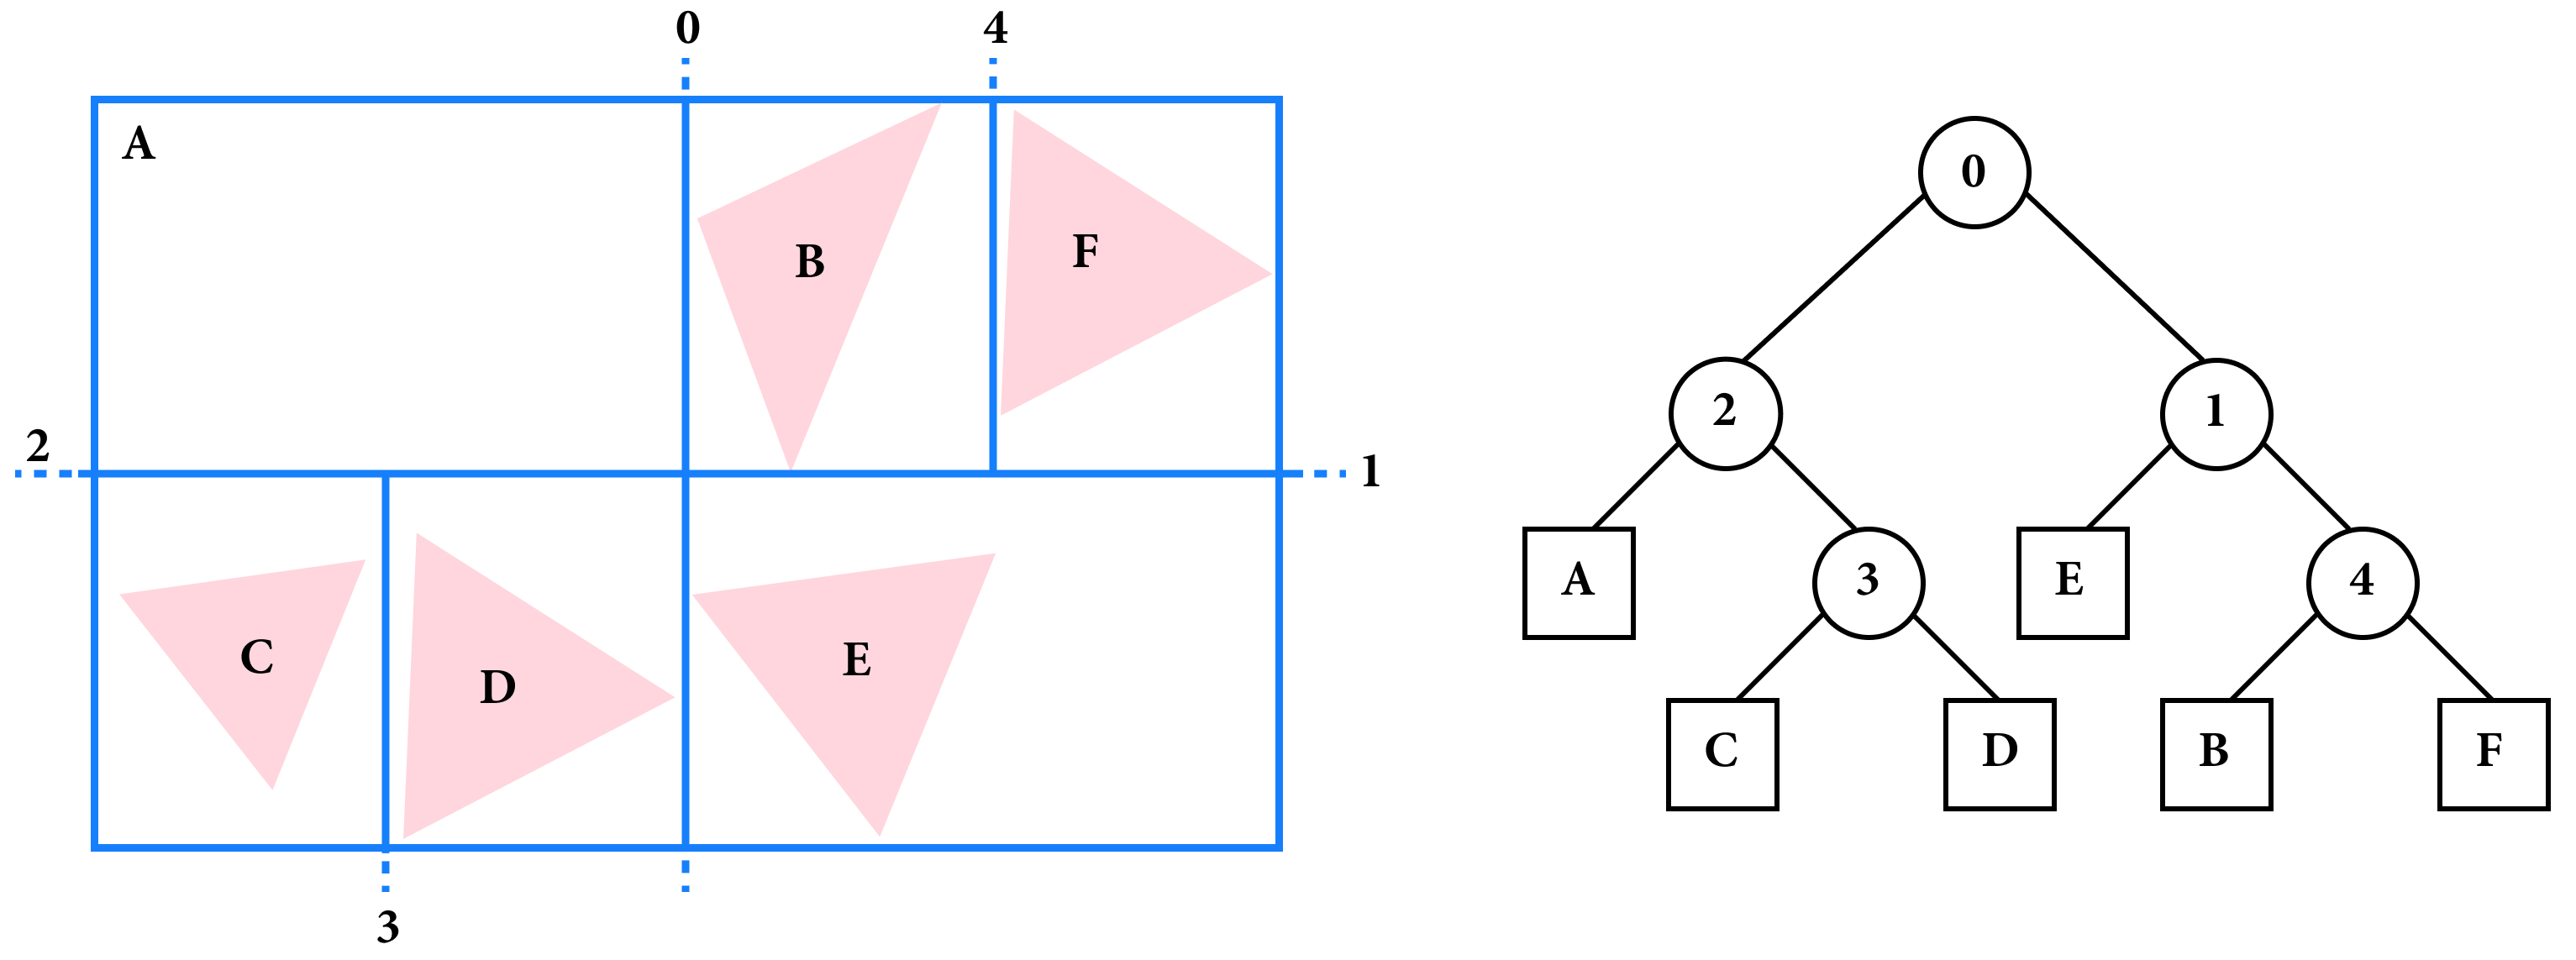
\includegraphics[width=\textwidth]{section4/4.3/bsp-tree-example.png}
	\end{center}
	\caption{Simple scene with a few triangles and a corresponding tree. Leaves are boxes and inner nodes are circles.}
	\label{sec4.3:example-kd-tree}
\end{figure}

\subsubsection{Traversing BSP trees}

A ray traverses a BSP tree by intersecting the ray with the split plane; therefore, giving a ray distance to the plane, allowing us to divide it into segments. The initial ray segment is computed by clipping the ray with the axis-aligned bounding box. We traverse a node if the ray segment overlays the node. Since the two-child nodes do not overlap, we can trivially classify which node is closer to the ray direction and traverse that node first. For the traversal algorithm, the children should be labeled as \textit{near} and \textit{far} child nodes, giving us three possible cases of traversal:

\begin{enumerate}
	\item Ray goes through near child only. (Figure \ref{sec4.3:near-child})
	\item Ray goes through far child only. (Figure \ref{sec4.3:far-child})
	\item Ray goes through the near child first followed by the far child. (Figure \ref{sec4.3:far-child})
\end{enumerate}

The near and far classification uses the direction of the ray and the position of the splitting plane. Therefore, it classifies the left node as near and the right node as far if the sign of the ray direction in the splitting axis is positive and vice versa if negative. Once we reach the terminal nodes, we can then search for the intersection of all the primitives in the node, if any.

\begin{figure}[ht]
	\centering
	\begin{subfigure}[b]{0.3\textwidth}
		\centering
		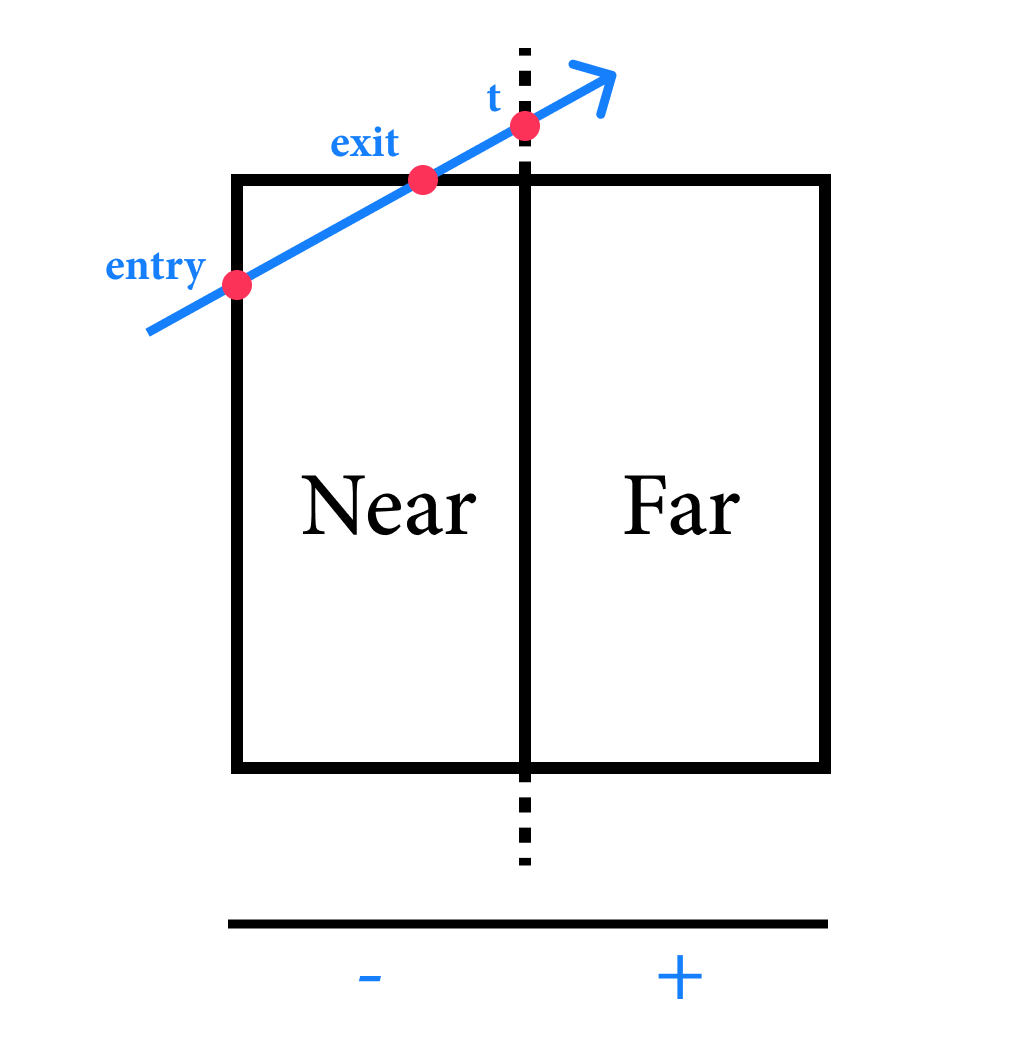
\includegraphics[width=\textwidth]{section4/4.3/near-intersection.png}
		\caption{Ray goes through near child only.}
		\label{sec4.3:near-child}
	\end{subfigure}
	\hfill
	\begin{subfigure}[b]{0.3\textwidth}
		\centering
		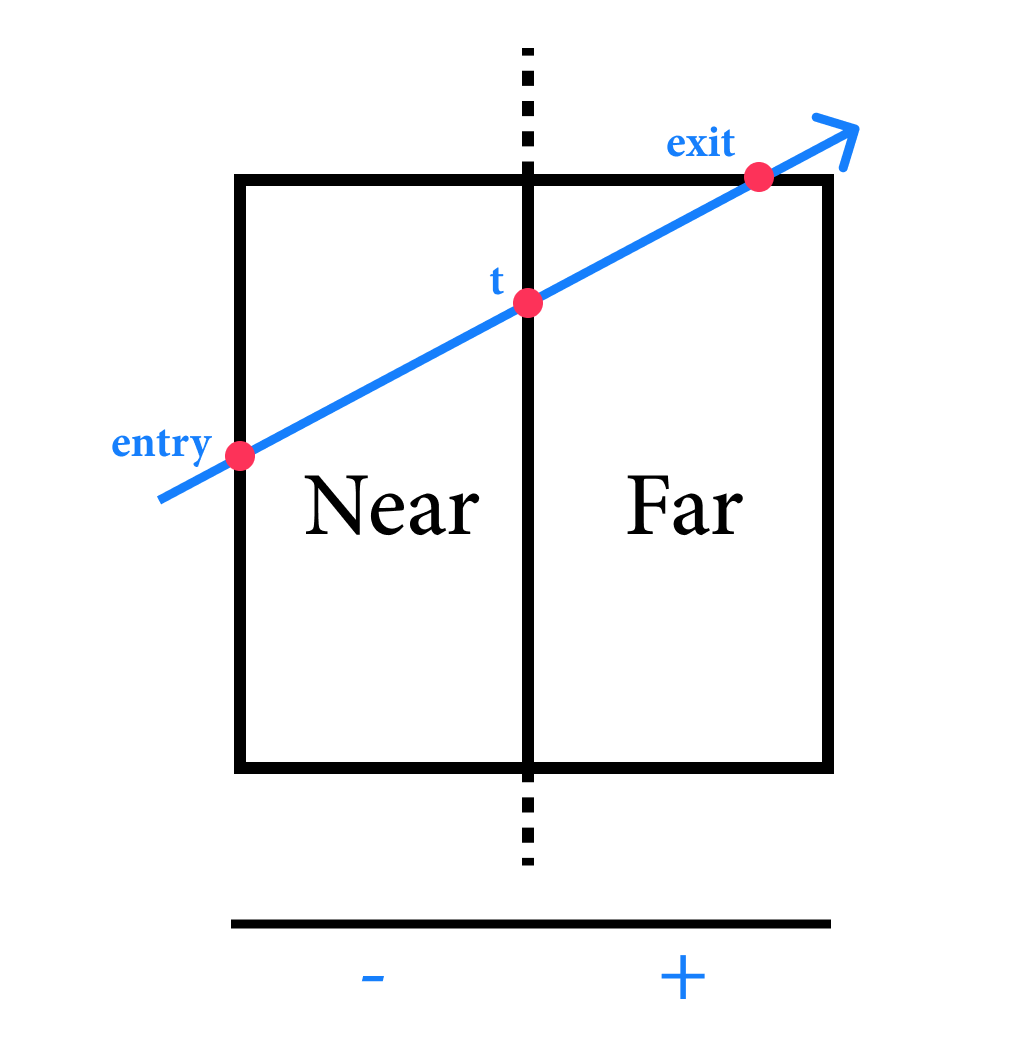
\includegraphics[width=\textwidth]{section4/4.3/middle-intersection.png}
		\caption{Ray goes through both children.}
		\label{sec4.3:both-children}
	\end{subfigure}
	\hfill
	\begin{subfigure}[b]{0.3\textwidth}
		\centering
		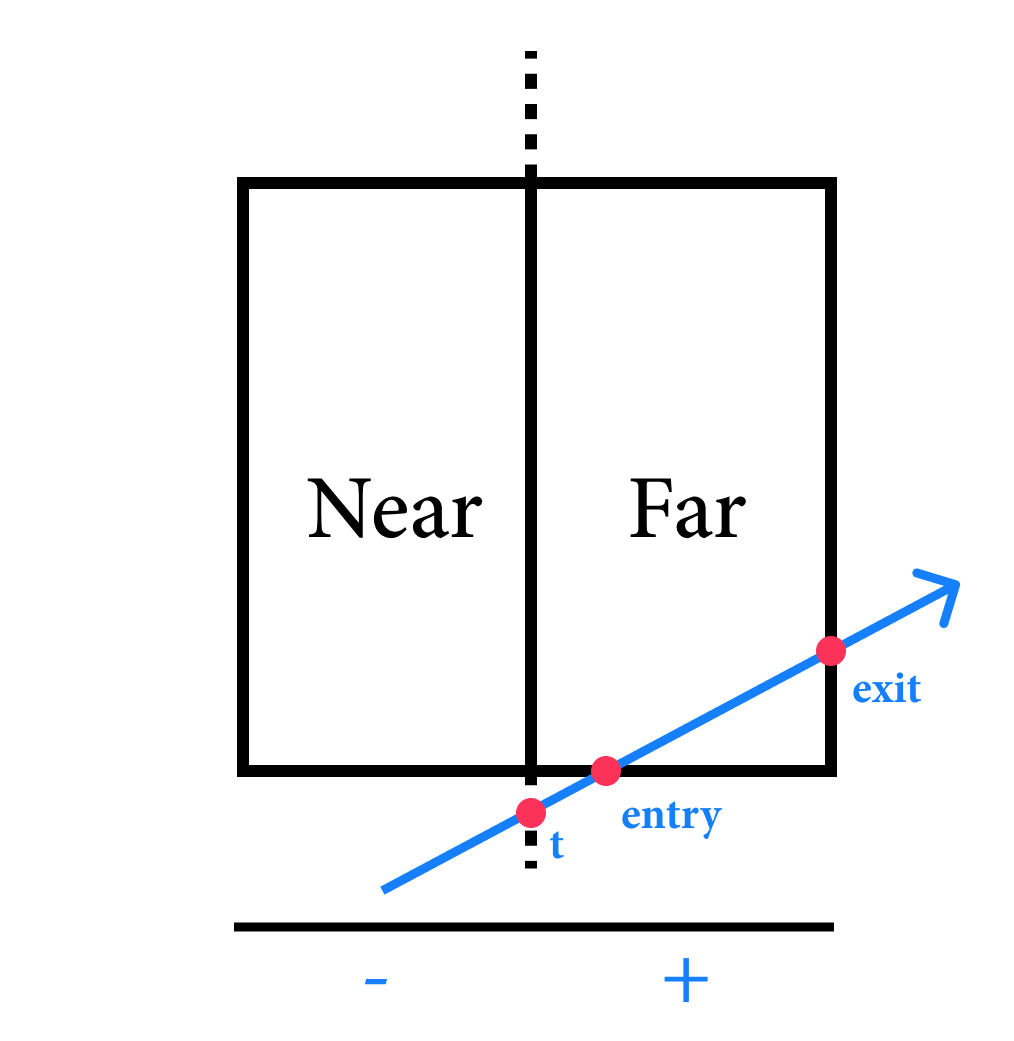
\includegraphics[width=\textwidth]{section4/4.3/far-intersection.png}
		\caption{Ray goes through near child only.}
		\label{sec4.3:far-child}
	\end{subfigure}
	\hfill
	\caption{Ray traversal cases.}
	\label{sec4.3:ray-traversal-cases}
\end{figure}

\subsection{Optimized CSG}

With all three optimizations from Sections \ref{section:classification-optimization}, \ref{section:bounding-boxes-optimization}, \ref{section:bsp-optimization}, we now have the building blocks for the optimized CSG algorithm. We can deconstruct this algorithm to a hierarchical pipeline of 4 elements. On the very top, we have our entire scene enclosed in a BSP tree. We then have constructively constructed geometries inside of this scene represented using two other BSP trees for their respective left and right geometries\footnote{In case the constructive solid only contains a single primitive element, then the tree is a simple tree of depth 1}. The trees can efficiently retrieve the closest intersections of their respective nodes, and have bounding boxes that allow quick tests of ray-solid intersections. Finally, upon retrieval of the ray intersections, the minimal hit algorithm allows for efficient and robust classification of these intersections. Even when nesting constructively generated geometries, one can hold definitions of each sub-tree for each sub-object. Hence, allowing for efficient evaluation of complex and nested geometries.  Such definition inherently means that each solid is reliable for its evaluation and can continually feed the correct and classified intersection information to its parent nodes. Therefore, skipping the step of gathering all evaluations and only processing them on the leaf nodes.

\section{Evaluation of the results}

There are three variants of the CSG method implemented in OpenRT. The first is the naive and brute force implementation which we refer to as $NaiCSG$. The second uses a binary space partition tree to solve the visible surface problem but still naively finds intersections inside the combinatorial geometry, which we will refer to as $BinCSG$. Finally, we'll introduce our optimized algorithm, which uses a binary space partition tree on the outside (solving the visible surface problem) and also inside each composite geometry to direct the rays towards the correct geometries, which we will refer to as $OptimCSG$. We consider each algorithm for all operations and a low, medium, and high viewport fill rate. We conduct three main tests. First, we assess how the rendering time develops to the complexity of the geometry. In this case, the complexity of the geometry is the number of polygons in the sphere meshes. The second test demonstrates how the spatial distribution of the scene affects the times for each of the algorithms. Therefore, helping us grasp how significant the viewport fill percentage changes each of these algorithms individually. We also run tests to count the number of intersection-tests performed by each variant at each pixel. The last test is based on the effect of a different number of nested geometries on the various algorithms while maintaining a relevantly similar viewport fill rate.

\subsection{Geometry Complexity Tests}

As previously mentioned, we conduct each of these tests on varying viewport fill rates. Figure \ref{sec5.1:viewport_range} shows the three main viewport ranges the tests. Different operations give different rates (e.g., difference and intersection will generally produce a less voluminous geometry); therefore, we account for this by determining the range in which the viewport fill wavers. We will refer to low, mid, and high viewport tests respectively as LVP, MVP, and HVP.

\begin{figure}[H] 
	\begin{center}
		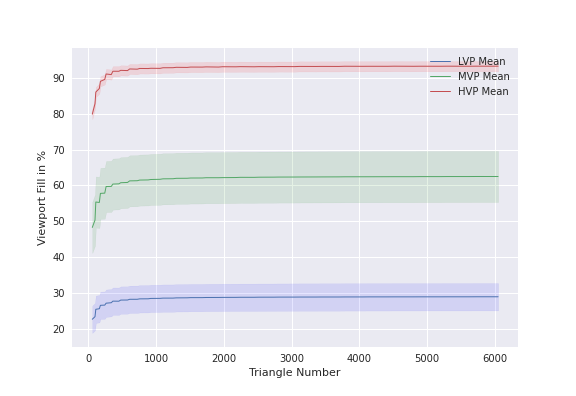
\includegraphics[width=0.7\textwidth]{section5/plots/view_port_final.png}
	\end{center}
	\caption{Range of view port rates on which the tests are conducted as the complexity of the geomtery increases. The area around the curve signifies the error by which the rate fluctuates.}
	\label{sec5.1:viewport_range}
\end{figure}


First, we will start by examining the different operations for the $NaiCSG$ implementation. Figures \ref{sec5.1:naive_operations_lvp} to \ref{sec5.1:naive_operations_hvp} show the performance of each operation in relation to the other. We don't discern any major difference between these operations because the procedure is naive and constantly performs the same amount of checks regardless of the operations. This variant is also insensitive to changing the viewport fill rate (Figure \ref{sec5.1:naive_operations}) since the computational time can't be reduced by ray-box tests.


\begin{figure}[H]
	\centering
	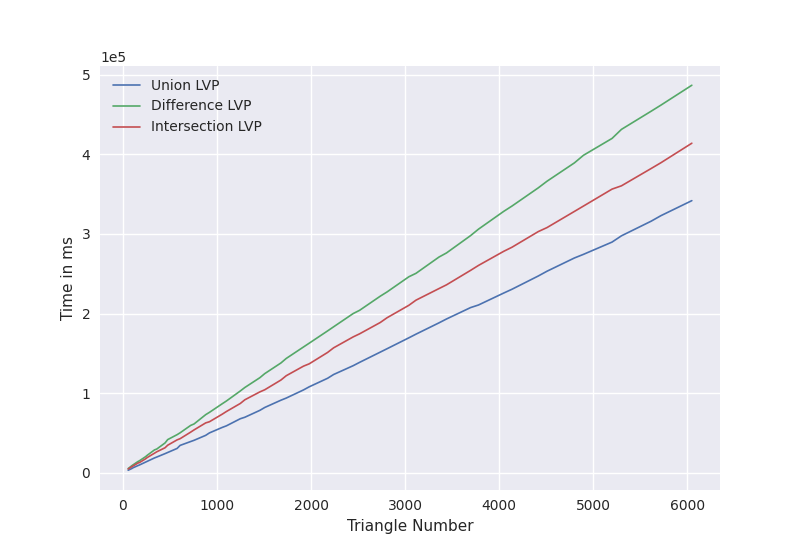
\includegraphics[width=0.7\textwidth]{section5/plots/naive_csg_lvp.png}
	\caption{$NaiCSG$ rendering time of different operations with respect to gradual increases in geometry complexity in a scene filling a small rate of the view port.}
	\label{sec5.1:naive_operations_lvp}
\end{figure}

\begin{figure}[H]
	\centering
	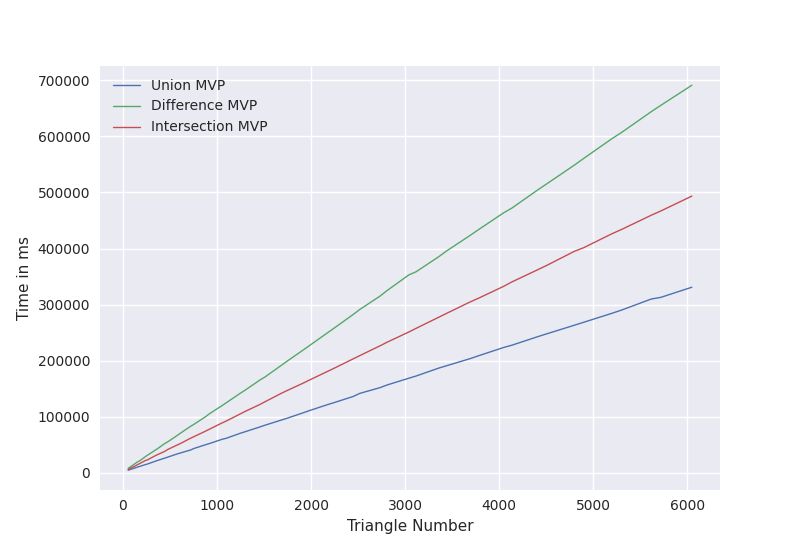
\includegraphics[width=0.7\textwidth]{section5/plots/naive_csg_mvp.png}
	\caption{$NaiCSG$ rendering time of different operations with respect to gradual increases in geometry complexity in a scene filling a medium rate of the view port.}
	\label{sec5.1:naive_operations_mvp}
\end{figure}

\begin{figure}[H]
	\centering
	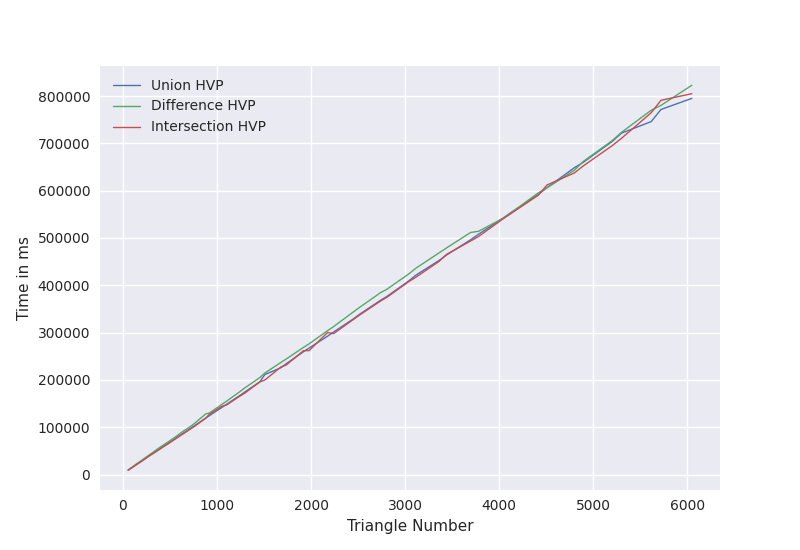
\includegraphics[width=0.7\textwidth]{section5/plots/naive_csg_hvp.png}
	\caption{$NaiCSG$ rendering time of different operations with respect to gradual increases in geometry complexity in a scene filling a high rate of the view port.}
	\label{sec5.1:naive_operations_hvp}
\end{figure}

\begin{figure}[H]
	\centering
	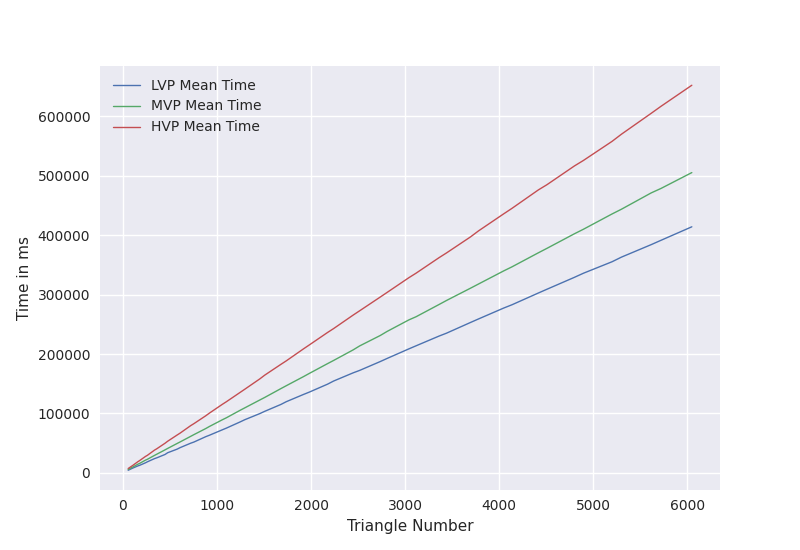
\includegraphics[width=0.7\textwidth]{section5/plots/naive_csg_mean.png}
	\caption{The $NaiCSG$ mean rendering time of the operations for the different view port fill rates.}
	\label{sec5.1:naive_operations}
\end{figure}

Second, we compare the rendering time of the $BinCSG$ variant. Figure \ref{sec5.1:bin_operations_lvp} to \ref{sec5.1:bin_operations_hvp} show the performance of each operation in relation to the other. In Figure \ref{sec5.1:bin_operations_lvp}, we notice a much more obvious discrepancy between the union operation and the two others. It is the case since the union operation creates a bigger geometry hence taking up a bigger portion of the viewport. As seen in Figure \ref{sec5.1:bin_operations_mvp} and \ref{sec5.1:bin_operations_hvp}, this gap closes up as bigger portions of the viewport are filled and time gained from the ray-box tests performed in $BinCSG$ become less useful. Figure \ref{sec5.1:bin_operations} demonstrates how the computational time of $BinCSG$ worsens depending on the spatial distribution in the scene.


\begin{figure}[H]
	\centering
	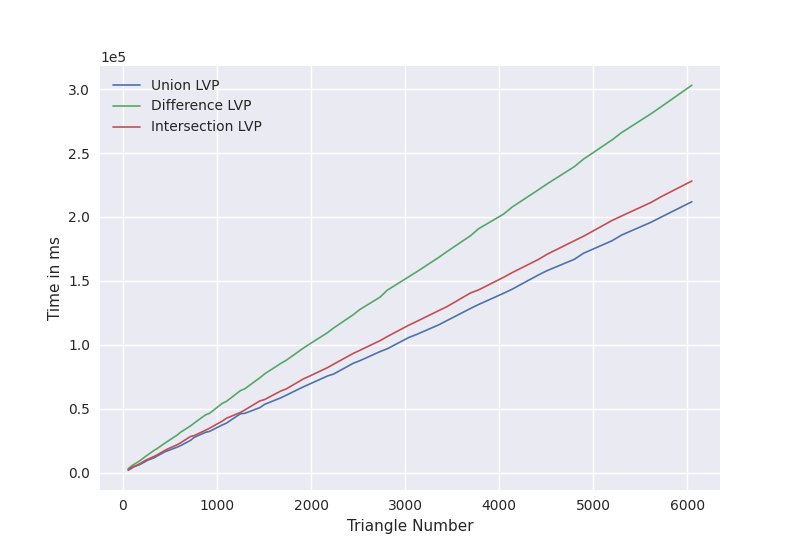
\includegraphics[width=0.7\textwidth]{section5/plots/bin_csg_lvp.png}
	\caption{$BinCSG$ rendering time of different operations with respect to gradual increases in geometry complexity in a scene filling a small rate of the view port.}
	\label{sec5.1:bin_operations_lvp}
\end{figure}

\begin{figure}[H]
	\centering
	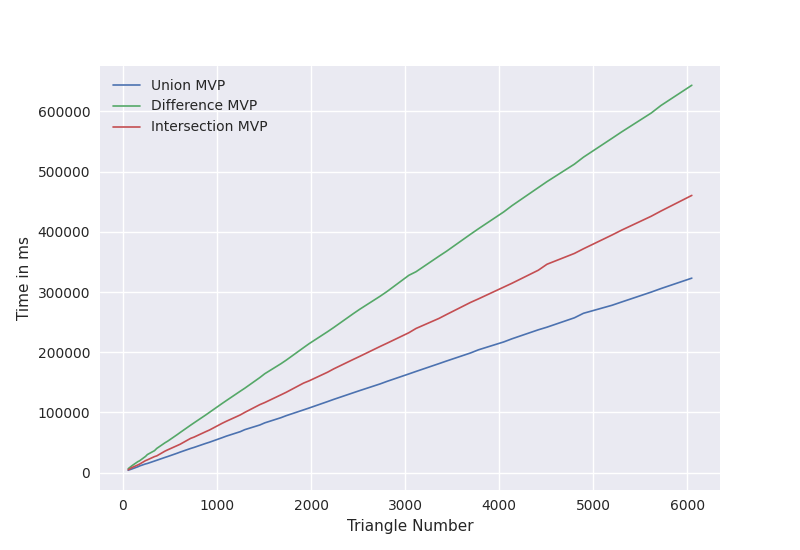
\includegraphics[width=0.7\textwidth]{section5/plots/bin_csg_mvp.png}
	\caption{$BinCSG$ rendering time of different operations with respect to gradual increases in geometry complexity in a scene filling a medium rate of the view port.}
	\label{sec5.1:bin_operations_mvp}
\end{figure}

\begin{figure}[H]
	\centering
	\includegraphics[width=0.7\textwidth]{section5/plots/bin_csg_hvp.png}
	\caption{$BinCSG$ rendering time of different operations with respect to gradual increases in geometry complexity in a scene filling a high rate of the view port.}
	\label{sec5.1:bin_operations_hvp}
\end{figure}

\begin{figure}[H]
	\centering
	\includegraphics[width=0.7\textwidth]{section5/plots/bin_csg_mean.png}
	\caption{The $BinCSG$ mean rendering time of the operations for the different view port fill rates.}
	\label{sec5.1:bin_operations}
\end{figure}

%todo update to match latest results.
We must also analyze the performance of $OptimCSG$ with the different operations. As we can see in Figures \ref{sec5.1:optim_operations_lvp} to \ref{sec5.1:optim_operations_hvp}, $OptimCSG$ shows a much more different performance in terms of the operations. The general curve is also not linear like $NaiCSG$ and $BinCSG$ but follows a rather logarithmic curve. The procedure also increases in time after an increase in the fill rate; however, nowhere as drastic as $BinCSG$.

\begin{figure}[H]
	\centering
	\includegraphics[width=0.7\textwidth]{section5/plots/optim_csg_lvp.png}
	\caption{$OptimCSG$ rendering time of different operations with respect to gradual increases in geometry complexity in a scene filling a small rate of the view port.}
	\label{sec5.1:optim_operations_lvp}
\end{figure}

\begin{figure}[H]
	\centering
	\includegraphics[width=0.7\textwidth]{section5/plots/optim_csg_mvp.png}
	\caption{$OptimCSG$ rendering time of different operations with respect to gradual increases in geometry complexity in a scene filling a medium rate of the view port.}
	\label{sec5.1:optim_operations_mvp}
\end{figure}

\begin{figure}[H]
	\centering
	\includegraphics[width=0.7\textwidth]{section5/plots/optim_csg_hvp.png}
	\caption{$OptimCSG$ rendering time of different operations with respect to gradual increases in geometry complexity in a scene filling a high rate of the view port.}
	\label{sec5.1:optim_operations_hvp}
\end{figure}
\begin{figure}[H]
	\centering
	\includegraphics[width=0.7\textwidth]{section5/plots/optim_csg_mean.png}
	\caption{The $OptimCSG$ mean rendering time of the operations for the different view port fill rates.}
	\label{sec5.1:bin_operations}
\end{figure}

Lastly, we compare the performance of these variants to each other. Figures \ref{sec5.1:geo_complexity_lvp} to \ref{sec5.1:geo_complexity_hvp} show the comparison of the different implementations with low, mid, and high viewport fills. As we can see, $OptimCSG$ outperforms both variants in all cases. $BinCSG$ does outperform $NaiCSG$ in a smaller scenes; however, it scales to the same computational time in more complex ones.

\begin{figure}[H]
	\centering
	\includegraphics[width=0.7\textwidth]{section5/plots/geo_complexity_lvp.png}
	\caption{Rendering time of different operations with respect to gradual increases in geometry complexity in a scene filling a small rate of the view port.}
	\label{sec5.1:geo_complexity_lvp}
\end{figure}

\begin{figure}[H]
	\centering
	\includegraphics[width=0.7\textwidth]{section5/plots/geo_complexity_mvp.png}
	\caption{Rendering time of different operations with respect to gradual increases in geometry complexity in a scene filling a medium rate of the view port.}
	\label{sec5.1:geo_complexity_mvp}
\end{figure}

\begin{figure}[H]
	\centering
	\includegraphics[width=0.7\textwidth]{section5/plots/geo_complexity_hvp.png}
	\caption{Rendering time of different operations with respect to gradual increases in geometry complexity in a scene filling a high rate of the view port.}
	\label{sec5.1:geo_complexity_hvp}
\end{figure}


We can explain these variations by the number of ray-primitive intersection tests performed by each variant. In the naive implementation, we check for all primitives for all the rays in the scene, which explains why it is not so case-dependent. In $BinCSG$, if the ray-box test is positive, it naively makes the ray-primitive intersections. $OptimCSG$ has a more directed approach as both the left and right geometries in the composite are also split up into smaller boxes and traversed efficiently. Figures \ref{sec5.1:test_count_naive} to \ref{sec5.1:test_count_optim} represent the number of intersection performed in a $1000 \times 1000$ pixel image with two spheres in the scene (Figure \ref{sec5.1:test_count_render}). In Figure \ref{sec5.1:test_count_naive} we can see that we continually make the same number of ray-primitive tests for each pixel. However, Figure \ref{sec5.1:test_count_bin} reveals how $BinCSG$ is capable of avoiding intersections toward the areas where the bounding box is not defined but still performs all tests in pixels overlapping it. Ultimately, $OptimCSG$ (Figure \ref{sec5.1:test_count_optim}) exhibits a much more efficient approach where the number of ray primitive intersections solely grows in areas dense with primitives.

\begin{figure}[H]
	\centering
	\includegraphics[width=0.6\textwidth]{section5/plots/union.png}
	\caption{The scene on which the number of intersections is counted.}
	\label{sec5.1:test_count_render}
\end{figure}

\begin{figure}[H]
	\centering
	\includegraphics[width=\textwidth]{section5/plots/surface_naive_union.png}
	\caption{Surface plot showing the number of ray-primitive tests on each pixel with $NaiCSG$}
	\label{sec5.1:test_count_naive}
\end{figure}

\begin{figure}[H]
	\centering
	\includegraphics[width=\textwidth]{section5/plots/surface_bin_union.png}
	\caption{Surface plot showing the number of ray-primitive tests on each pixel with $BinCSG$}
	\label{sec5.1:test_count_bin}
\end{figure}

\begin{figure}[H]
	\centering
	\includegraphics[width=\textwidth]{section5/plots/surface_optim_union.png}
	\caption{Surface plot showing the number of ray-primitive tests on each pixel with $OptimCSG$}
	\label{sec5.1:test_count_optim}
\end{figure}


\subsection{Nesting Tests}

An important aspect to observe is how the algorithms handle the nesting of many geometries together. Here we attempt to maintain a relatively steady viewport fill rate as we increase the number of nests. Figure \ref{sec5.2:test_nesting_rates} shows how the viewport fill rate fluctuates with the mean value while conducting these tests.

\begin{figure}[H]
	\centering
	\includegraphics[width=0.6\textwidth]{section5/plots/test_nesting_rates.png}
	\caption{Range of view port rates on which the tests are conducted as the number of nests increases.}
	\label{sec5.2:test_nesting_rates}
\end{figure}


Figure \ref{sec5.2:test_nesting} portrays the different performances of each variant. As expected, the naive time grows linearly as we use more geometries. $BinCSG$ is also somewhat linear but is expected to scale to the same time as the naive if we increase the viewport fill rate. On the other hand $OptimCSG$ still follows a logarithmic trend when nesting. 

\begin{figure}[H]
	\centering
	\includegraphics[width=0.6\textwidth]{section5/plots/test_nesting.png}
	\caption{Performance of the different variants in comparison to each other when nesting more geometries together.}
	\label{sec5.2:test_nesting}
\end{figure}



\section{Conclusion \& Future Work}


The observed results in the previous section lay a foundation for accelerating the performance of complex geometrical modeling using CSG in real applications. We have briefly covered the general mathematical foundation of constructively generated geometry. We then introduced the generic idea behind constructive solid geometry and the algebraic rules applied to it. Later, we introduced different optimizations used to push the performance of each operation. Last, we compared each variant and understood its time complexity. There are still various means of possibly improving the performance of the proposed solution while still maintaining a balance of generality and robustness. I outline a few issues with the proposed algorithm and possible future research directions in accelerated ray tracing of constructive solid geometry in this section.

The first encountered issue is artifacts created by the numeric stability issues in classification. When classifying using the surface normals, we will run into the issue where the dot product of the ray direction and the normal is near zero (vectors are orthogonal). Hence, leading to certain artifacts emerging near the boundaries of the geometries of edges. The described issue can be solved using a sampler which would increase the number of rays shot in the neighborhood of a pixel and estimate a better shading result. This solution is already plausible in OpenRT.

The second limitation is that the geometries must have consistently oriented normals to understand intersections. While all primitives and solids constructed inside OpenRT guarantee this property, meshes imported from the outside could potentially lead to issues. However, one can solve this by implementing an extra scan when constructing solids or passing them to a composite to verify and modify the surface normals when needed. Algorithms that allow for fast checks of consistent normal orientation are readily available \cite{normal_orientation}.

Many improvements are also possible in alignment with the work established in this paper. The first is extending the binary space partitioning tree algorithm to be more efficient in building and traversing. Such a change can bring drastic improvements to the performance and handle much more complex scenes. Automated stopping criteria are a way to let each solid deterministically choose which stopping criteria work best, particularly in BREPs.

Second, this research heavily focused on acceleration with CPU-based ray tracing. Many solutions to extend the system to a GPU exist, and such benefits could make the algorithm gain from the ever-increasing performance of the graphics hardware.

Conversion algorithms from constructively defined solids to BREPs are detrimental as well. Conversion allows for faster computations and ease of use. If we can translate a constructively generated geometry to a BREP,  we can increase performance, and final geometries would no longer rely on a recursive evaluation. One can then also use the optimized triangle operations for faster computations and rendering. The solution is especially appealing since we can divide complex geometries into smaller models to unify later.

Applying textures to constructive solid geometry is also an area of interest. We could achieve the latter with a few different flavors. Automatic texture mapping is one of them. The goal is of automatic texture mapping is to produce texture coordinates for geometries that don't possess any. One could use a sphere, cube, or any other map to generate these texture coordinates. Therefore, enabling the use of different textures on each of the constructively generated geometries.	 The texture coordinate generation function can also be specified separately for each geometry from the user.

Topics such as the reconstruction of constructive solid geometry trees using unsupervised neural networks are also interesting. \cite{ucsgnet_ml} produced models that allow for fast and accurate reconstruction of CSG trees from images. Such an advancement would make the possibility of combining a multitude of geometrical resources simpler. Additionally, combining this with the conversion to a boundary representation makes such a possibility more appealing.
  

\newpage
%\bibliographystyle{unsrt}
%\bibliography{bsc-sample}
\printbibliography

\end{document}